% Options for packages loaded elsewhere
\PassOptionsToPackage{unicode}{hyperref}
\PassOptionsToPackage{hyphens}{url}
%
\documentclass[
  man,floatsintext]{apa6}
\usepackage{amsmath,amssymb}
\usepackage{iftex}
\ifPDFTeX
  \usepackage[T1]{fontenc}
  \usepackage[utf8]{inputenc}
  \usepackage{textcomp} % provide euro and other symbols
\else % if luatex or xetex
  \usepackage{unicode-math} % this also loads fontspec
  \defaultfontfeatures{Scale=MatchLowercase}
  \defaultfontfeatures[\rmfamily]{Ligatures=TeX,Scale=1}
\fi
\usepackage{lmodern}
\ifPDFTeX\else
  % xetex/luatex font selection
\fi
% Use upquote if available, for straight quotes in verbatim environments
\IfFileExists{upquote.sty}{\usepackage{upquote}}{}
\IfFileExists{microtype.sty}{% use microtype if available
  \usepackage[]{microtype}
  \UseMicrotypeSet[protrusion]{basicmath} % disable protrusion for tt fonts
}{}
\makeatletter
\@ifundefined{KOMAClassName}{% if non-KOMA class
  \IfFileExists{parskip.sty}{%
    \usepackage{parskip}
  }{% else
    \setlength{\parindent}{0pt}
    \setlength{\parskip}{6pt plus 2pt minus 1pt}}
}{% if KOMA class
  \KOMAoptions{parskip=half}}
\makeatother
\usepackage{xcolor}
\usepackage{color}
\usepackage{fancyvrb}
\newcommand{\VerbBar}{|}
\newcommand{\VERB}{\Verb[commandchars=\\\{\}]}
\DefineVerbatimEnvironment{Highlighting}{Verbatim}{commandchars=\\\{\}}
% Add ',fontsize=\small' for more characters per line
\usepackage{framed}
\definecolor{shadecolor}{RGB}{248,248,248}
\newenvironment{Shaded}{\begin{snugshade}}{\end{snugshade}}
\newcommand{\AlertTok}[1]{\textcolor[rgb]{0.94,0.16,0.16}{#1}}
\newcommand{\AnnotationTok}[1]{\textcolor[rgb]{0.56,0.35,0.01}{\textbf{\textit{#1}}}}
\newcommand{\AttributeTok}[1]{\textcolor[rgb]{0.13,0.29,0.53}{#1}}
\newcommand{\BaseNTok}[1]{\textcolor[rgb]{0.00,0.00,0.81}{#1}}
\newcommand{\BuiltInTok}[1]{#1}
\newcommand{\CharTok}[1]{\textcolor[rgb]{0.31,0.60,0.02}{#1}}
\newcommand{\CommentTok}[1]{\textcolor[rgb]{0.56,0.35,0.01}{\textit{#1}}}
\newcommand{\CommentVarTok}[1]{\textcolor[rgb]{0.56,0.35,0.01}{\textbf{\textit{#1}}}}
\newcommand{\ConstantTok}[1]{\textcolor[rgb]{0.56,0.35,0.01}{#1}}
\newcommand{\ControlFlowTok}[1]{\textcolor[rgb]{0.13,0.29,0.53}{\textbf{#1}}}
\newcommand{\DataTypeTok}[1]{\textcolor[rgb]{0.13,0.29,0.53}{#1}}
\newcommand{\DecValTok}[1]{\textcolor[rgb]{0.00,0.00,0.81}{#1}}
\newcommand{\DocumentationTok}[1]{\textcolor[rgb]{0.56,0.35,0.01}{\textbf{\textit{#1}}}}
\newcommand{\ErrorTok}[1]{\textcolor[rgb]{0.64,0.00,0.00}{\textbf{#1}}}
\newcommand{\ExtensionTok}[1]{#1}
\newcommand{\FloatTok}[1]{\textcolor[rgb]{0.00,0.00,0.81}{#1}}
\newcommand{\FunctionTok}[1]{\textcolor[rgb]{0.13,0.29,0.53}{\textbf{#1}}}
\newcommand{\ImportTok}[1]{#1}
\newcommand{\InformationTok}[1]{\textcolor[rgb]{0.56,0.35,0.01}{\textbf{\textit{#1}}}}
\newcommand{\KeywordTok}[1]{\textcolor[rgb]{0.13,0.29,0.53}{\textbf{#1}}}
\newcommand{\NormalTok}[1]{#1}
\newcommand{\OperatorTok}[1]{\textcolor[rgb]{0.81,0.36,0.00}{\textbf{#1}}}
\newcommand{\OtherTok}[1]{\textcolor[rgb]{0.56,0.35,0.01}{#1}}
\newcommand{\PreprocessorTok}[1]{\textcolor[rgb]{0.56,0.35,0.01}{\textit{#1}}}
\newcommand{\RegionMarkerTok}[1]{#1}
\newcommand{\SpecialCharTok}[1]{\textcolor[rgb]{0.81,0.36,0.00}{\textbf{#1}}}
\newcommand{\SpecialStringTok}[1]{\textcolor[rgb]{0.31,0.60,0.02}{#1}}
\newcommand{\StringTok}[1]{\textcolor[rgb]{0.31,0.60,0.02}{#1}}
\newcommand{\VariableTok}[1]{\textcolor[rgb]{0.00,0.00,0.00}{#1}}
\newcommand{\VerbatimStringTok}[1]{\textcolor[rgb]{0.31,0.60,0.02}{#1}}
\newcommand{\WarningTok}[1]{\textcolor[rgb]{0.56,0.35,0.01}{\textbf{\textit{#1}}}}
\usepackage{graphicx}
\makeatletter
\def\maxwidth{\ifdim\Gin@nat@width>\linewidth\linewidth\else\Gin@nat@width\fi}
\def\maxheight{\ifdim\Gin@nat@height>\textheight\textheight\else\Gin@nat@height\fi}
\makeatother
% Scale images if necessary, so that they will not overflow the page
% margins by default, and it is still possible to overwrite the defaults
% using explicit options in \includegraphics[width, height, ...]{}
\setkeys{Gin}{width=\maxwidth,height=\maxheight,keepaspectratio}
% Set default figure placement to htbp
\makeatletter
\def\fps@figure{htbp}
\makeatother
\setlength{\emergencystretch}{3em} % prevent overfull lines
\providecommand{\tightlist}{%
  \setlength{\itemsep}{0pt}\setlength{\parskip}{0pt}}
\setcounter{secnumdepth}{-\maxdimen} % remove section numbering
% Make \paragraph and \subparagraph free-standing
\ifx\paragraph\undefined\else
  \let\oldparagraph\paragraph
  \renewcommand{\paragraph}[1]{\oldparagraph{#1}\mbox{}}
\fi
\ifx\subparagraph\undefined\else
  \let\oldsubparagraph\subparagraph
  \renewcommand{\subparagraph}[1]{\oldsubparagraph{#1}\mbox{}}
\fi
\newlength{\cslhangindent}
\setlength{\cslhangindent}{1.5em}
\newlength{\csllabelwidth}
\setlength{\csllabelwidth}{3em}
\newlength{\cslentryspacingunit} % times entry-spacing
\setlength{\cslentryspacingunit}{\parskip}
\newenvironment{CSLReferences}[2] % #1 hanging-ident, #2 entry spacing
 {% don't indent paragraphs
  \setlength{\parindent}{0pt}
  % turn on hanging indent if param 1 is 1
  \ifodd #1
  \let\oldpar\par
  \def\par{\hangindent=\cslhangindent\oldpar}
  \fi
  % set entry spacing
  \setlength{\parskip}{#2\cslentryspacingunit}
 }%
 {}
\usepackage{calc}
\newcommand{\CSLBlock}[1]{#1\hfill\break}
\newcommand{\CSLLeftMargin}[1]{\parbox[t]{\csllabelwidth}{#1}}
\newcommand{\CSLRightInline}[1]{\parbox[t]{\linewidth - \csllabelwidth}{#1}\break}
\newcommand{\CSLIndent}[1]{\hspace{\cslhangindent}#1}
\ifLuaTeX
\usepackage[bidi=basic]{babel}
\else
\usepackage[bidi=default]{babel}
\fi
\babelprovide[main,import]{english}
% get rid of language-specific shorthands (see #6817):
\let\LanguageShortHands\languageshorthands
\def\languageshorthands#1{}
% Manuscript styling
\usepackage{upgreek}
\captionsetup{font=singlespacing,justification=justified}

% Table formatting
\usepackage{longtable}
\usepackage{lscape}
% \usepackage[counterclockwise]{rotating}   % Landscape page setup for large tables
\usepackage{multirow}		% Table styling
\usepackage{tabularx}		% Control Column width
\usepackage[flushleft]{threeparttable}	% Allows for three part tables with a specified notes section
\usepackage{threeparttablex}            % Lets threeparttable work with longtable

% Create new environments so endfloat can handle them
% \newenvironment{ltable}
%   {\begin{landscape}\centering\begin{threeparttable}}
%   {\end{threeparttable}\end{landscape}}
\newenvironment{lltable}{\begin{landscape}\centering\begin{ThreePartTable}}{\end{ThreePartTable}\end{landscape}}

% Enables adjusting longtable caption width to table width
% Solution found at http://golatex.de/longtable-mit-caption-so-breit-wie-die-tabelle-t15767.html
\makeatletter
\newcommand\LastLTentrywidth{1em}
\newlength\longtablewidth
\setlength{\longtablewidth}{1in}
\newcommand{\getlongtablewidth}{\begingroup \ifcsname LT@\roman{LT@tables}\endcsname \global\longtablewidth=0pt \renewcommand{\LT@entry}[2]{\global\advance\longtablewidth by ##2\relax\gdef\LastLTentrywidth{##2}}\@nameuse{LT@\roman{LT@tables}} \fi \endgroup}

% \setlength{\parindent}{0.5in}
% \setlength{\parskip}{0pt plus 0pt minus 0pt}

% Overwrite redefinition of paragraph and subparagraph by the default LaTeX template
% See https://github.com/crsh/papaja/issues/292
\makeatletter
\renewcommand{\paragraph}{\@startsection{paragraph}{4}{\parindent}%
  {0\baselineskip \@plus 0.2ex \@minus 0.2ex}%
  {-1em}%
  {\normalfont\normalsize\bfseries\itshape\typesectitle}}

\renewcommand{\subparagraph}[1]{\@startsection{subparagraph}{5}{1em}%
  {0\baselineskip \@plus 0.2ex \@minus 0.2ex}%
  {-\z@\relax}%
  {\normalfont\normalsize\itshape\hspace{\parindent}{#1}\textit{\addperi}}{\relax}}
\makeatother

% \usepackage{etoolbox}
\makeatletter
\patchcmd{\HyOrg@maketitle}
  {\section{\normalfont\normalsize\abstractname}}
  {\section*{\normalfont\normalsize\abstractname}}
  {}{\typeout{Failed to patch abstract.}}
\patchcmd{\HyOrg@maketitle}
  {\section{\protect\normalfont{\@title}}}
  {\section*{\protect\normalfont{\@title}}}
  {}{\typeout{Failed to patch title.}}
\makeatother

\usepackage{xpatch}
\makeatletter
\xapptocmd\appendix
  {\xapptocmd\section
    {\addcontentsline{toc}{section}{\appendixname\ifoneappendix\else~\theappendix\fi\\: #1}}
    {}{\InnerPatchFailed}%
  }
{}{\PatchFailed}
\keywords{meta-analysis, monte carlo simulations, power analysis\newline\indent Word count: 7869}
\usepackage{csquotes}
\usepackage{setspace}
\captionsetup[figure]{font={stretch=1,footnotesize}}
\usepackage{float}
\usepackage{orcidlink}
\newcommand{\rev}[1]{\textcolor{red}{#1}}
\ifLuaTeX
  \usepackage{selnolig}  % disable illegal ligatures
\fi
\IfFileExists{bookmark.sty}{\usepackage{bookmark}}{\usepackage{hyperref}}
\IfFileExists{xurl.sty}{\usepackage{xurl}}{} % add URL line breaks if available
\urlstyle{same}
\hypersetup{
  pdftitle={Understanding meta-analysis through data simulation with applications to power analysis},
  pdfauthor={Filippo Gambarota 1 \& Gianmarco Altoè 1},
  pdflang={en-EN},
  pdfkeywords={meta-analysis, monte carlo simulations, power analysis},
  hidelinks,
  pdfcreator={LaTeX via pandoc}}

\title{Understanding meta-analysis through data simulation with applications to power analysis}
\author{Filippo Gambarota \orcidlink{0000-0002-6666-1747}\textsuperscript{1} \& Gianmarco Altoè \orcidlink{0000-0003-1154-9528}\textsuperscript{1}}
\date{}


\shorttitle{Simulating meta-analysis}

\authornote{

The authors made the following contributions. Filippo Gambarota \orcidlink{0000-0002-6666-1747}: Conceptualization, Methodology, Formal Analysis, Software, Writing -- Original Draft; Gianmarco Altoè \orcidlink{0000-0003-1154-9528}: Conceptualization, Methodology, Writing - Review \& Editing, Supervision.

Correspondence concerning this article should be addressed to Filippo Gambarota \orcidlink{0000-0002-6666-1747}, Via Venezia 8, 35131 Padova (PD). E-mail: \href{mailto:filippo.gambarota@unipd.it}{\nolinkurl{filippo.gambarota@unipd.it}}

}

\affiliation{\vspace{0.5cm}\textsuperscript{1} Department of Developmental and Social Psychology, University of Padova, Italy}

\abstract{%
Meta-analysis is a powerful tool to combine evidence from existing literature. Despite several introductory and advanced materials about organizing, conducting, and reporting a meta-analysis, to our knowledge, there are no introductive materials about simulating the most common meta-analysis models. Data simulation is essential for developing and validating new statistical models and procedures. Furthermore, data simulation is a powerful educational tool for understanding a statistical method. In this tutorial, we show how to simulate equal-effects, random-effects, and meta-regression models and illustrate how to estimate statistical power. In the supplementary materials, we extended these simulations also for multilevel and multivariate models. All materials associated with this article can be accessed on Open Science Framework (\url{https://osf.io/54djn/}).
}



\begin{document}
\maketitle

\setcounter{secnumdepth}{5}

\hypertarget{introduction}{%
\section{Introduction}\label{introduction}}

\begin{quote}
``If you do not simulate it, you have not understood it.''
\end{quote}

A meta-analysis is an essential tool for combining knowledge from multiple studies quantitatively. Meta-analysis is commonly used together with a systematic review of the literature. The meta-analysis has several advantages. Firstly, it allows combining evidence from multiple studies assigning more weight to studies with lower estimation variability. Then using meta-regression, it is possible to include variables (i.e., moderators) to explain the observed heterogeneity (Borenstein, Hedges, Higgins, \& Rothstein, 2009, pp. 187--203). More recently, location-scale models have been developed to include predictors also on the residual heterogeneity (i.e., Viechtbauer \& López-López, 2022). Finally, considering the replication crisis, there are statistical methods to determine the presence and extent of the publication bias. Despite the advantages, meta-analysis implementation is not always straightforward, especially for complex data structures. Additionally, the fact that there are several introductory and advanced resources to understand meta-analysis (Borenstein et al., 2009; Harrer, Cuijpers, Furukawa, \& Ebert, 2021; Schmid, Stijnen, \& White, 2022), to our knowledge, there are no introductory resources about how to simulate realistic meta-analytic data.

Simulating data has several advantages because it requires understanding the statistical method and the data-generation process. Furthermore, data simulation is the primary tool when it comes to evaluating a new analysis method, estimating the statistical power, or understanding the long-run behavior of our data generation process (Gelman \& Hill, 2006, pp. 155--176; Gelman, Hill, \& Vehtari, 2020, pp. 69--76; Ingalls, 2011). A recent paper by DeBruine and Barr (2021), which deeply inspired the current work, proposed a stimulating way to understand linear mixed-effects models via data simulation. Simulating data is also a powerful educational tool within this framework.

For these reasons, this work aims to introduce the basic concepts of meta-analysis and Monte Carlo simulations for equal-effects, random-effects, and meta-regression models with applications also to statistical power calculation. In the first section, we will introduce basic concepts of the meta-analysis that are useful for setting up the simulation. We will evaluate the effect size, variance calculation, and the equal vs.~random effects model distinction. Then we will describe how to simulate data for these models and simulate a meta-regression with categorical and numerical predictors. Finally, we will introduce the power analysis extending the previous examples to estimate the statistical power. We used the R statistical programming language (version 4.3.1; R Core Team, 2023).

The aim of the tutorial is not to provide a complete theoretical introduction to meta-analysis but rather to present core topics using a simulation-based approach. Readers experienced in conducting meta-analyses can benefit from the proposed approach in terms of simulation setup and coding strategies. Readers without prior experience in meta-analysis can benefit both from the theoretical introduction and the simulation approach. However, for a more comprehensive overview of meta-analysis topics the reader may refer to meta-analysis textbooks (Borenstein et al., 2009; e.g., Harrer, Cuijpers, \& Ebert, 2019)

We assume the reader is familiar with the basic concepts of R, but core functions will be explained. Code and materials are available on the OSF repository (\url{https://osf.io/54djn/}). A theoretical introduction, simulation examples for multivariate and multilevel models, and more details about the coding approach are available in the supplementary materials.

\hypertarget{meta-analysis-introduction}{%
\subsection{Meta-analysis introduction}\label{meta-analysis-introduction}}

The meta-analysis is a statistical procedure to combine multiple studies (i.e., \emph{primary studies}) into a single statistical analysis (Borenstein et al., 2009). The idea is that combining numerous preliminary studies improve the estimation of a particular phenomenon more efficiently compared to conducting a single study. In statistical terms, the concept of the meta-analysis is to switch the statistical unit from the single participant or observation (i.e., \emph{level 1}) to the study (i.e., \emph{level 2}). Given that some studies will give more information because their estimation variability is smaller (e.g., higher sample size), the meta-analysis combines the studies assigning more weight as a function of the precision (i.e., the inverse of the variance).

As an example that will be used throughout the paper, we consider the efficacy of memory training in improving memory performance during a cognitive task. The typical primary study will collect data from a group of participants receiving the memory training (\emph{experimental group}) and another group receiving a control treatment (\emph{control group}). The focus of the meta-analysis is collecting multiple studies with similar aims and methods and estimating the average effect of memory training. Despite differences in the type of cognitive task or experimental setup, each primary study collects an \emph{experimental group} (\(n_{T}\)) and \emph{control group} (\(n_{C}\)) and computes the average performance (\emph{experimental group} \(\overline T\) and \emph{control group} \(\overline C\)) and standard deviations (\emph{experimental group} \(s_{T}\) and \emph{control group}
\(s_{C}\)).

\hypertarget{effect-size-and-variance}{%
\subsubsection{Effect size and variance}\label{effect-size-and-variance}}

The first step of a meta-analysis is to extract information from included studies. This common measure should give an immediate idea of the direction (i.e., the treatment improves or reduces performance) and the size of the effect. Standardized effect size measures (see Lakens, 2013 for an overview), such as the Standardized Mean Difference (SMD), which could be estimated by Cohen's \(d\) (Cohen, 1988) or the Pearson correlation coefficient \(\rho\) which could be calculated using the associated sample estimator \emph{r} are commonly used to compare heterogeneous outcome variables\footnote{ When using bounded effect sizes such as the Pearson correlation, Fisher Z-transformation is commonly used (Borenstein et al., 2009, pp. 41--43)}. If all studies used the same raw measure, such as reaction times, it is possible to directly meta-analyze the studies without standardizing e.g.~using the unstandardized mean difference (UMD, Borenstein et al., 2009, pp. 21--24).

As reported in the previous section, beyond the effect size of each study, we need to assign a weight according to the precision. For this reason, we need to calculate the sampling variability of the effect size or the raw measure that will represent the estimation precision. Each raw or standardized effect size measure (e.g., raw mean difference, Cohen's \(d\), and Pearson's correlation) has a different formula to calculate the sampling variability. The idea is to choose the appropriate measure considering the study design (e.g., between vs.~within-subjects) and available information and find the proper formula to compute the sampling variability. In addition, there are formulas and approaches to convert from one effect size measure to another (Borenstein et al., 2009; Lakens, 2013; Lipsey \& Wilson, 2001).\footnote{See also the blog post by James Pustejovsky (\href{https://www.jepusto.com/alternative-formulas-for-the-smd/}{www.jepusto.com/alternative-formulas-for-the-smd}) for a general method to compute the sampling variability for standardized mean difference measures.} Usually, the effect size sampling variability depends mainly on the sample size that determines the weight assigned during the meta-analytic estimation.

\hypertarget{equal-vs-fixed-vs-random-effects-model}{%
\subsubsection{Equal vs fixed vs random-effects model}\label{equal-vs-fixed-vs-random-effects-model}}

The core of a meta-analysis is combining the results of multiple studies giving more weight to studies that provide a more precise effect estimation. We can find essentially three meta-analysis models: the equal-effects, the fixed-effects, and the random-effects model (Hedges \& Vevea, 1998; Laird \& Mosteller, 1990). The \emph{equal-effects} model assumes that each study included in the meta-analysis is a more or less precise estimation of the true underlying effect (\(\theta\)). In other terms, we are assuming that there is no variability (i.e., heterogeneity) among true effect sizes. On the other side, suppose some study-level characteristics (e.g., participants' age, sex, or socioeconomic status) or the experimental paradigm (e.g., type of memory task or difficulty) could impact the treatment effect. In this case, we have true variability (i.e., heterogeneity) among studies. The \emph{random-effects} model assumes a distribution of real effects with mean \(\mu_{\theta}\) and variance \(\tau^{2}\) thus estimating the heterogeneity. Finally, the \emph{fixed-effects} model estimate the average effect of the included pool of studies ignoring the presence of heterogeneity. While the distinction between the equal and fixed-effects model is theoretical, the estimated model is the exactly the same\footnote{See \href{https://wviechtb.github.io/metafor/reference/misc-models.html}{wviechtb.github.io/metafor/reference/misc-models.html} for a detailed explanation}. The \emph{random-effects} model assumes and estimates heterogeneity among effect sizes leading to different model parameters. From an inferential point of view, the \emph{random-effects} model provides unconditional inference to the population of effect sizes while the \emph{fixed-effects} model estimates the average effect of the selected studies and not population-level parameters. The \emph{equal-effects} model assumes a single true population effect to be estimated. Figure \ref{fig:img-equal-vs-random} depicts the theoretical distinction between the equal and random-effects model. In the presence of heterogeneity, we can include moderators (e.g., the type of experimental setup) into a meta-regression model to explain the effect size heterogeneity. An interesting proposal to combine evidence from these different models into a single analysis is called Bayesian model-averaged meta-analysis (Berkhout, Haaf, Gronau, Heck, \& Wagenmakers, 2023; Gronau, Heck, Berkhout, Haaf, \& Wagenmakers, 2021). However, this model is beyond the scope of the tutorial.

\scriptsize

\begin{figure}[H]

{\centering \includegraphics[width=0.8\linewidth]{C:/Users/user/Documents/work/shared-projects/simulating-meta-analysis/documents/output/paper_files/figure-latex/img-equal-vs-random-1} 

}

\caption{The difference between the assumptions of the \emph{equal} and \emph{random-effects model}. Each distribution depicts the sampling distribution of \(k = 4\) hypothetical studies (\(i = 1\), \(2\), \ldots, \(4\)) with a certain observed effect size \(y_{i}\) (pink squares), sampling variability \(\sigma_{\epsilon_i}^{2}\) and the 95\% confidence interval (black segment). The \emph{equal-effects} plot on the left suggests that each observed effect size has the same underlying true effect \(\theta\) (each distribution has the same mean) with a different degree of precision (e.g., Study 1 is more precise than Study 3). In practice, each study has a different observed effect size where studies with high precision (i.e., narrow sampling distributions) will be close to the real effect (\(\theta\)). The \emph{random-effects model} on the right suggests that beyond the error term (\(\epsilon_{i}\)), each real effect size is composed of a fixed part (now \(\mu_{\theta}\)) and a random part (\(\delta_{i}\)) sampled from a normal distribution with mean zero and variance \(\tau^{2}\). When \(\tau^{2}\) is zero, the random-effects reduces to a equal-effects model.}\label{fig:img-equal-vs-random}
\end{figure}

\normalsize

\hypertarget{simulation}{%
\section{Simulation}\label{simulation}}

\hypertarget{monte-carlo-simulations}{%
\subsection{Monte Carlo simulations}\label{monte-carlo-simulations}}

The Monte Carlo methods are controlled experiments (Gentle, 2009). Given a set of fixed parameters, probability distributions, and the possibility of generating random numbers, it is possible to simulate the behavior of an empirical system. Monte Carlo simulations are used for statistical and mathematical problems that cannot be solved analytically.

A straightforward example regards estimating the sampling variability of the mean difference. When calculating the mean difference between two samples, we estimate the true mean difference at the population level with a certain degree of error (i.e., the standard error of the mean difference). The central limit theorem states that the difference between the means of two random samples (\(\overline{X}\) and \(\overline{Y}\)) is approximately normally distributed with mean \(\mu_{x} - \mu_{y}\) and standard error \(\sqrt{\frac{\sigma^2_x}{{n_x}} + \frac{\sigma^2_y}{{n_y}}}\). The same results can be obtained using Monte Carlo simulations using the following procedure:

\begin{enumerate}
\def\labelenumi{\arabic{enumi}.}
\tightlist
\item
  Generating two random samples from two normal distributions with a fixed mean difference
\item
  Calculating the mean difference
\item
  Repeating the same process, many times
\item
  Calculate the standard deviation of the simulated values
\end{enumerate}

Using the method, we are estimating via simulation the standard deviation of the sampling distribution of the mean difference (i.e., the standard error of the mean difference). Increasing the number of simulations will produce more stable results.

\scriptsize

\begin{Shaded}
\begin{Highlighting}[]
\FunctionTok{set.seed}\NormalTok{(}\DecValTok{123}\NormalTok{) }\CommentTok{\# seed for simulation to ensure the reproducibility of results}
\NormalTok{es }\OtherTok{\textless{}{-}} \FloatTok{0.5} \CommentTok{\# real mean difference in the populations}
\NormalTok{sigma }\OtherTok{\textless{}{-}} \DecValTok{1} \CommentTok{\# real standard deviations in the population}
\NormalTok{n }\OtherTok{\textless{}{-}} \DecValTok{30} \CommentTok{\# sample size for both groups}
\NormalTok{nsims }\OtherTok{\textless{}{-}} \FloatTok{1e5} \CommentTok{\# number of simulations = 100000}

\CommentTok{\# simulates the sampling distribution of the mean difference}
\NormalTok{d\_mc }\OtherTok{\textless{}{-}} \FunctionTok{replicate}\NormalTok{(nsims, }\AttributeTok{expr =}\NormalTok{ \{}
\NormalTok{  g1 }\OtherTok{\textless{}{-}} \FunctionTok{rnorm}\NormalTok{(}\AttributeTok{n =}\NormalTok{ n, }\AttributeTok{mean =}\NormalTok{ es, }\AttributeTok{sd =}\NormalTok{ sigma)}
\NormalTok{  g2 }\OtherTok{\textless{}{-}} \FunctionTok{rnorm}\NormalTok{(}\AttributeTok{n =}\NormalTok{ n, }\AttributeTok{mean =} \DecValTok{0}\NormalTok{, }\AttributeTok{sd =}\NormalTok{ sigma)}
  \FunctionTok{mean}\NormalTok{(g1) }\SpecialCharTok{{-}} \FunctionTok{mean}\NormalTok{(g2) }\CommentTok{\# calculates the sample mean difference and returns the value}
\NormalTok{\})}

\CommentTok{\# analytical standard error of the mean difference}
\NormalTok{se\_an }\OtherTok{\textless{}{-}} \FunctionTok{sqrt}\NormalTok{(sigma}\SpecialCharTok{\^{}}\DecValTok{2}\SpecialCharTok{/}\NormalTok{n }\SpecialCharTok{+}\NormalTok{ sigma}\SpecialCharTok{\^{}}\DecValTok{2}\SpecialCharTok{/}\NormalTok{n)}

\CommentTok{\# monte{-}carlo standard error of the mean difference}
\NormalTok{se\_mc }\OtherTok{\textless{}{-}} \FunctionTok{sd}\NormalTok{(d\_mc)}
\end{Highlighting}
\end{Shaded}

\normalsize

The standard error estimated solving analytically is 0.26 and using the Monte Carlo simulation we arrive at the same result (i.e., 0.26).

\hypertarget{simulation-setup}{%
\subsection{Simulation setup}\label{simulation-setup}}

This tutorial uses several R packages for the simulations, meta-analysis fitting, and figures/tables. For the data manipulation, we used the \emph{tidyverse} (Wickham, 2023) package. For the models fitting we used the \emph{metafor} (Viechtbauer, 2010) package. For figures and tables the \emph{ggplot2} (Wickham et al., 2023) or the \texttt{metafor::forest()} function, \emph{kableExtra} (Zhu, 2021) and \emph{papaja} (Aust \& Barth, 2022) packages. We set the \texttt{seed} for reproducibility of the simulation environment.

\scriptsize

\begin{Shaded}
\begin{Highlighting}[]
\FunctionTok{library}\NormalTok{(dplyr) }\CommentTok{\# for data manipulation (within tidyverse)}
\FunctionTok{library}\NormalTok{(tidyr) }\CommentTok{\# for data manipulation (within tidyverse)}
\FunctionTok{library}\NormalTok{(metafor) }\CommentTok{\# for meta{-}analysis models fitting}
\FunctionTok{library}\NormalTok{(purrr) }\CommentTok{\# for *apply like functions (within tidyverse)}
\NormalTok{seed }\OtherTok{\textless{}{-}} \DecValTok{2023} \CommentTok{\# general seed for all simulations}
\end{Highlighting}
\end{Shaded}

\normalsize

Before diving into the specific simulations, in this section, we define the common aspects of all simulations in the following sections. The current paper focuses on the \emph{two-level}, \emph{equal,} and \emph{random-effects} models. All the examples refer to primary studies that assess the efficacy of a treatment by comparing a control and an experimental group. In simulation studies where the purpose is not evaluating effect size estimators, it is convenient to simulate unstandardized effect size measures (see Viechtbauer, 2005, 2007). The estimator is unbiased thus not requiring small sample correction (Hedges, 1981; e.g., Hedges, 1989). Furthermore, the effect size and the sampling variance are independent. Similar to the simulation approach by Viechtbauer (2005, 2007) the \emph{experimental} group (\(T\)) and \emph{control} groups \(C\) are sampled from normal distributions respectively \(T_i \sim \mathcal{N}(\Delta, 1)\) and \(C_i \sim \mathcal{N}(0, 1)\) where \(\Delta\) is the unstandardized mean difference (UMD). The UMD and the sampling variance are calculated using Equations \eqref{eq:effsize} and \eqref{eq:effsizevar} where \(y\) is the estimated value of \(\Delta\).

\begin{align}
\begin{gathered}
D = \overline{T} - \overline{C}
\label{eq:effsize}
\end{gathered}
\end{align}

\begin{align}
\begin{gathered}
\sigma_{\epsilon D}^{2} = \frac{s^2_T}{n_T} + \frac{s^2_C}{n_C}
\label{eq:effsizevar}
\end{gathered}
\end{align}

We can use the following algorithm implemented in the \texttt{sim\_study()} function to simulate a single study. Before using the \texttt{sim\_study()}
function, we can create a data frame for the simulation using the \texttt{make\_data()} function\footnote{This function is a simple wrapper of \texttt{data.frame()} that given the number of studies and other variables create the data structure for the simulation.}. Table \ref{tab:sim-data-example-tab} depicts an example of the \texttt{make\_data()} output.

\begin{enumerate}
\def\labelenumi{\arabic{enumi}.}
\tightlist
\item
  Choose a \(\Delta\), \(n_{T}\), and \(n_{C}\) value.
\item
  Simulate \(n_{T}\) observations from a Gaussian distribution with \(\mu = \Delta\) and \(\sigma^{2} = 1\) and \(n_{T}\) observations from a Gaussian distribution with \(\mu = 0\) and \(\sigma^{2} = 1\). In this way, the expected difference between groups will be \(\Delta\) and the expected variance for each group is 1.
\item
  Calculate the observed effect size \(y\) and the sampling variance \(\sigma_{\epsilon}^{2}\).
\end{enumerate}

The simulation approach can be easily extended calculating a standardized effect size measures (e.g., Cohens' \(d\) Cohen, 1988) and the corresponding sampling variance. For example, after generating data for the two groups the mean difference can be standardized using the pooled standard deviation and applying the appropriate correction (Hedges, 1981; e.g., Hedges, 1989).

\scriptsize

\begin{Shaded}
\begin{Highlighting}[]

\NormalTok{make\_data }\OtherTok{\textless{}{-}} \ControlFlowTok{function}\NormalTok{(k, }\AttributeTok{nt =} \ConstantTok{NULL}\NormalTok{, }\AttributeTok{nc =} \ConstantTok{NULL}\NormalTok{, ...)\{}
\NormalTok{  params }\OtherTok{\textless{}{-}} \FunctionTok{c}\NormalTok{(}\FunctionTok{as.list}\NormalTok{(}\FunctionTok{environment}\NormalTok{()), }\FunctionTok{list}\NormalTok{(...))}
\NormalTok{  cols }\OtherTok{\textless{}{-}}\NormalTok{ params[}\SpecialCharTok{!}\FunctionTok{sapply}\NormalTok{(params, is.null) }\SpecialCharTok{\&} \FunctionTok{names}\NormalTok{(params) }\SpecialCharTok{!=} \StringTok{"k"}\NormalTok{]}
\NormalTok{  dat }\OtherTok{\textless{}{-}} \FunctionTok{data.frame}\NormalTok{(}
    \AttributeTok{id =} \DecValTok{1}\SpecialCharTok{:}\NormalTok{params}\SpecialCharTok{$}\NormalTok{k}
\NormalTok{  )}
  \ControlFlowTok{if}\NormalTok{(}\FunctionTok{length}\NormalTok{(cols) }\SpecialCharTok{!=} \DecValTok{0}\NormalTok{)\{}
\NormalTok{    dat }\OtherTok{\textless{}{-}} \FunctionTok{cbind}\NormalTok{(dat, cols)}
\NormalTok{  \}}
  \FunctionTok{return}\NormalTok{(dat)}
\NormalTok{\}}
\end{Highlighting}
\end{Shaded}

\normalsize

\scriptsize

\begin{Shaded}
\begin{Highlighting}[]

\NormalTok{sim\_study }\OtherTok{\textless{}{-}} \ControlFlowTok{function}\NormalTok{(es, nt, }\AttributeTok{nc =} \ConstantTok{NULL}\NormalTok{, }\AttributeTok{aggregate =} \ConstantTok{TRUE}\NormalTok{)\{}
  \ControlFlowTok{if}\NormalTok{(}\FunctionTok{is.null}\NormalTok{(nc)) nc }\OtherTok{\textless{}{-}}\NormalTok{ nt}
  \CommentTok{\# generate from normal distribution}
\NormalTok{  yc }\OtherTok{\textless{}{-}} \FunctionTok{rnorm}\NormalTok{(nc, }\DecValTok{0}\NormalTok{, }\DecValTok{1}\NormalTok{)}
\NormalTok{  yt }\OtherTok{\textless{}{-}} \FunctionTok{rnorm}\NormalTok{(nt, es, }\DecValTok{1}\NormalTok{)}
  
  \CommentTok{\# effect size}
\NormalTok{  yi }\OtherTok{\textless{}{-}}\NormalTok{ (}\FunctionTok{mean}\NormalTok{(yt) }\SpecialCharTok{{-}} \FunctionTok{mean}\NormalTok{(yc))}
  
  \CommentTok{\# sampling variance}
\NormalTok{  vi }\OtherTok{\textless{}{-}} \FunctionTok{var}\NormalTok{(yt)}\SpecialCharTok{/}\NormalTok{nt }\SpecialCharTok{+} \FunctionTok{var}\NormalTok{(yt)}\SpecialCharTok{/}\NormalTok{nc}
  
  \ControlFlowTok{if}\NormalTok{(}\SpecialCharTok{!}\NormalTok{aggregate)\{}
    \CommentTok{\# return raw data}
    \FunctionTok{data.frame}\NormalTok{(}\AttributeTok{id =} \DecValTok{1}\SpecialCharTok{:}\NormalTok{(nc }\SpecialCharTok{+}\NormalTok{ nt),}
               \AttributeTok{group =} \FunctionTok{rep}\NormalTok{(}\FunctionTok{c}\NormalTok{(}\StringTok{"c"}\NormalTok{, }\StringTok{"t"}\NormalTok{), }\FunctionTok{c}\NormalTok{(nc, nt)),}
               \AttributeTok{y =} \FunctionTok{c}\NormalTok{(yc, yt))}
\NormalTok{  \}}\ControlFlowTok{else}\NormalTok{\{}
    \CommentTok{\# compute effect size}
    \FunctionTok{data.frame}\NormalTok{(yi, vi)}
\NormalTok{  \}}
\NormalTok{\}}

\NormalTok{sim\_studies }\OtherTok{\textless{}{-}} \ControlFlowTok{function}\NormalTok{(..., }\AttributeTok{data =} \ConstantTok{NULL}\NormalTok{)\{}
  \CommentTok{\# ... (dots) are the arguments passed to mapply, with the order required by sim\_study}
\NormalTok{  res }\OtherTok{\textless{}{-}} \FunctionTok{mapply}\NormalTok{(sim\_study, ..., }\AttributeTok{SIMPLIFY =} \ConstantTok{FALSE}\NormalTok{)}
  \CommentTok{\# everything to a dataframe}
\NormalTok{  res }\OtherTok{\textless{}{-}}\NormalTok{ dplyr}\SpecialCharTok{::}\FunctionTok{bind\_rows}\NormalTok{(res)}
  
  \ControlFlowTok{if}\NormalTok{(}\SpecialCharTok{!}\FunctionTok{is.null}\NormalTok{(data))\{}
    \CommentTok{\# attach to the original dataset}
    \FunctionTok{cbind}\NormalTok{(data, res)}
\NormalTok{  \}}\ControlFlowTok{else}\NormalTok{\{}
\NormalTok{    res}
\NormalTok{  \}}
\NormalTok{\}}
\end{Highlighting}
\end{Shaded}

\normalsize

The \texttt{es} is the true effect size (\(\mu_{\theta}\) for the random-effects model and \(\theta\) for the equal-effects model), \texttt{nc} and \texttt{nt} are the sample size for the control and experimental group, \texttt{aggregate} controls if returning the effect size and the corresponding sampling variance or the participant-level data. We can generate a single study with the desired parameters with this function. A suggestion for each simulation step is to generate a large \(n\) to reduce the sampling error and check the recovery of simulated parameters. This is a general strategy that can be applied to every simulation. The \texttt{sim\_studies()} function will iterate through variables in the \texttt{...} argument creating the meta-analysis data frame. The \texttt{mapply()} function is clearly explained in the supplementary materials.

The following code simulates a single study with \(n = 10000\) and check the estimated mean and standard deviation.

\scriptsize

\begin{Shaded}
\begin{Highlighting}[]
\FunctionTok{set.seed}\NormalTok{(seed)}
\FunctionTok{sim\_study}\NormalTok{(}\AttributeTok{es =} \FloatTok{0.3}\NormalTok{, }\AttributeTok{nc =} \DecValTok{10000}\NormalTok{, }\AttributeTok{nt =} \DecValTok{10000}\NormalTok{, }\AttributeTok{aggregate =} \ConstantTok{FALSE}\NormalTok{)}
\end{Highlighting}
\end{Shaded}

\normalsize

\scriptsize

\normalsize

The control group has a mean of -0.008 (SD = 0.996) and the experimental group has a mean of 0.306 (SD = 1.013) which are remarkably close to the simulated values.

Using the \texttt{sim\_study()} function multiple times (with the appropriate adjustments) we can generate a series of studies simulating a data set for a meta-analysis (using the \texttt{sim\_studies()} function). After each example, we will compute the appropriate model (e.g., \emph{equal} or \emph{random-effects}) using the \texttt{metafor} package (Viechtbauer, 2010) to check the recovery of simulated parameters\footnote{ By default \texttt{metafor} use the Wald \emph{z} test on model parameters but other inference methods are available e.g.~the Knapp and Hartung (2003) method by setting \texttt{test="knha"} within the \texttt{rma()} function. This method is useful especially when the number of studies is low (see \href{https://wviechtb.github.io/metafor/reference/misc-recs.html}{wviechtb.github.io/metafor/reference/misc-recs.html} for more details)}. Table \ref{tab:notation-tab} summarizes the notation used in simulations and code in equations and code.

\scriptsize

\begin{Shaded}
\begin{Highlighting}[]
\NormalTok{k }\OtherTok{\textless{}{-}} \DecValTok{30} \CommentTok{\# number of studies}
\NormalTok{n }\OtherTok{\textless{}{-}} \DecValTok{20} \CommentTok{\# number of participants per group, per study}
\NormalTok{es }\OtherTok{\textless{}{-}} \FloatTok{0.3} \CommentTok{\# real effect size}
\NormalTok{sim }\OtherTok{\textless{}{-}} \FunctionTok{make\_data}\NormalTok{(}\AttributeTok{k =}\NormalTok{ k, }\AttributeTok{nt =}\NormalTok{ n, }\AttributeTok{nc =}\NormalTok{ n, }\AttributeTok{es =}\NormalTok{ es)}
\end{Highlighting}
\end{Shaded}

\normalsize

\scriptsize

\begin{table}[H]

\begin{center}
\begin{threeparttable}

\caption{\label{tab:sim-data-example-tab}Example of data generated with the \texttt{make\_data()} function. The \texttt{id} column is the identifier for each study.}

\small{

\begin{tabular}{llll}
\toprule
id & \multicolumn{1}{c}{nt} & \multicolumn{1}{c}{nc} & \multicolumn{1}{c}{es}\\
\midrule
1 & 20 & 20 & 0.3\\
2 & 20 & 20 & 0.3\\
... & ... & ... & ...\\
29 & 20 & 20 & 0.3\\
30 & 20 & 20 & 0.3\\
\bottomrule
\end{tabular}

}

\end{threeparttable}
\end{center}

\end{table}

\normalsize

\scriptsize

\begin{table}[H]

\begin{center}
\begin{threeparttable}

\caption{\label{tab:notation-tab}Variables in the data-generating model and associated R code.}

\begin{tabular}{lll}
\toprule
Equation & \multicolumn{1}{c}{Code} & \multicolumn{1}{c}{Description}\\
\midrule
$\theta$ & \texttt{theta} & Equal-effects model true effect size\\
$\mu_{\theta}$ & \texttt{mu\_theta} & Random-effects model true effect size\\
$\tau^2$ & \texttt{tau2} & Effect sizes heterogeneity\\
$\tau^2_r$ & \texttt{tau2r} & Residual effect sizes heterogeneity\\
$\overline{T}, \overline{C}$ & \texttt{} & Mean of the experimental/control group\\
$s_{T, C}$ & \texttt{} & Standard deviation of the experimental/control group\\
$n_{T, C}$ & \texttt{nt, nc} & Sample size of the experimental/control group\\
$y_i$ & \texttt{yi} & Observed effect size\\
$\sigma_{\epsilon_i}^{2}$ & \texttt{vi} & Observed sampling variance\\
$\delta_i$ & \texttt{deltai} & Random effect for the study i\\
$\beta_0$ & \texttt{b0} & Meta-regression intercept\\
$\beta_1$ & \texttt{b1} & Meta-regression slope\\
$k$ & \texttt{k} & Number of studies\\
$\epsilon_i$ & \texttt{} & Sampling error for the study i\\
\bottomrule
\addlinespace
\end{tabular}

\begin{tablenotes}[para]
\normalsize{\textit{Note.} The \texttt{yi} and \texttt{vi} notation for the observed effect size ($y_i$) and sampling variance ($\sigma_{\epsilon_i}^{2}$) has been used to be consistent with the \texttt{metafor} notation.}
\end{tablenotes}

\end{threeparttable}
\end{center}

\end{table}

\normalsize

\hypertarget{equal-effects-model}{%
\subsection{Equal-effects model}\label{equal-effects-model}}

The most basic model to simulate is the \emph{equal-effects model} (EE). As reported in the previous sections, the \emph{equal-effects model} assumes the presence of a single true effect (\(\theta\)) and the observed variability is caused by each effect size being a more or less imprecise estimation of the true effect. In other words, the only source of variability is the sampling variability that depends on the variance of the primary studies (i.e., the sample size). Equations \eqref{eq:equal-effects-model1} and \eqref{eq:equal-effects-model2} formalize the \emph{equal-effects} model.

\begin{align}
\begin{gathered}
y_i = \theta + \epsilon_i
\label{eq:equal-effects-model1}
\end{gathered}
\end{align}

\begin{align}
\begin{gathered}
\epsilon_i \sim \mathcal{N}(0,\sigma_{\epsilon_i}^{2})
\label{eq:equal-effects-model2}
\end{gathered}
\end{align}

Each observed effect size (\(y_{i}\)) is composed of the real effect size \(\theta\) plus an error term (\(\epsilon_{i}\)) that is sampled from a normal distribution with \(\mu = 0\) and \(\sigma^{2} = \sigma_{\epsilon_i}^{2}\) (i.e., the known sampling variance of the study \(i\)). As demonstrated in Equation \eqref{eq:effsize}, the increase in sample size will decrease the sampling variability. A study with a extremely large sample size will essentially have \(\theta\) as the observed effect size. Since we are sampling participants' level data, the error component is already included in the \texttt{sim\_study()} function. To simulate this model in R we can just call the \texttt{sim\_study()} multiple times according to the number of desired studies (\(k\)). In addition, we simulate that each primary study will have a sample size of \(n = 20\) for both groups. We will discuss later the appropriateness of this assumption.

\scriptsize

\begin{Shaded}
\begin{Highlighting}[]
\FunctionTok{set.seed}\NormalTok{(seed)}
\NormalTok{k }\OtherTok{\textless{}{-}} \DecValTok{30} \CommentTok{\# number of studies}
\NormalTok{n }\OtherTok{\textless{}{-}} \DecValTok{20} \CommentTok{\# number of participants per group, per study}
\NormalTok{theta }\OtherTok{\textless{}{-}} \FloatTok{0.3} \CommentTok{\# real effect size}

\NormalTok{sim }\OtherTok{\textless{}{-}} \FunctionTok{make\_data}\NormalTok{(}\AttributeTok{k =}\NormalTok{ k, }\AttributeTok{nt =}\NormalTok{ n, }\AttributeTok{nc =}\NormalTok{ n, }\AttributeTok{es =}\NormalTok{ theta)}
\NormalTok{sim }\OtherTok{\textless{}{-}} \FunctionTok{sim\_studies}\NormalTok{(sim}\SpecialCharTok{$}\NormalTok{es, sim}\SpecialCharTok{$}\NormalTok{nc, sim}\SpecialCharTok{$}\NormalTok{nt, }\AttributeTok{data =}\NormalTok{ sim) }\CommentTok{\# simulated data}
\NormalTok{res }\OtherTok{\textless{}{-}} \FunctionTok{rma}\NormalTok{(}\AttributeTok{yi =}\NormalTok{ yi, }\AttributeTok{vi =}\NormalTok{ vi, }\AttributeTok{method =} \StringTok{"EE"}\NormalTok{, }\AttributeTok{data =}\NormalTok{ sim)}
\end{Highlighting}
\end{Shaded}

\normalsize

We are using the \(\theta\) parameter to generate random data using the \texttt{sim\_study()} function that will introduce the random error component \(\epsilon_{i}\). Then we can fit the \emph{equal-effects} meta-analysis model with the \texttt{rma} function and \texttt{method\ =\ "EE"} of the \texttt{metafor} package. The parameter we are estimating is \(\theta\) which is close to our simulation value (see Table \ref{tab:res-equal-effects}). Increasing the number of studies (\(k\)) and/or the number of participants in each study (\(n\)) will improve estimation reducing the standard error.

\scriptsize

\begin{table}[H]

\caption{\label{tab:res-equal-effects}Summary of the simulated equal-effects model. The only estimated parameter is the average effect \(\theta\) (\(\beta\)) with the standard error, 95\% confidence interval, and the Wald z-test. The z-test evaluates the null hypothesis that the real effect equals zero.}
\centering
\fontsize{9}{11}\selectfont
\begin{tabular}[t]{ccccc}
\toprule
 & $\beta$ & 95\% CI & z & p\\
\midrule
overall & 0.347 (SE = 0.056) & $[0.237, 0.456]$ & 6.223 & < 0.001\\
\bottomrule
\multicolumn{5}{l}{\textsuperscript{} $k = 30$}\\
\end{tabular}
\end{table}

\normalsize

Increasing the sample size for each study will increase the estimation precision thus the variability among studies will be reduced. This can be easily demonstrated by simulating studies with a high sample size as reported in Figure \ref{fig:equal-effects-high-low-precision}. As the sample size increases the only source of variability (i.e., the error component \(\epsilon_{i}\)) is close to zero so each study is closer to the true simulated value.

\scriptsize

\begin{figure}[H]

{\centering \includegraphics[width=0.8\linewidth]{C:/Users/user/Documents/work/shared-projects/simulating-meta-analysis/documents/output/paper_files/figure-latex/equal-effects-high-low-precision-1} 

}

\caption{Forest plots of two simulated \emph{equal-effects models}. On the left, the simulated model has \(nt,nc = 30\) for each included study while on the right the sample size for each study is \(nt,nc = 500\). Given that the data were generated under a \emph{equal-effects model}, when the sample size is high (on the right) each study is aligned on the real effect size because the error component (\(\epsilon_{i}\)) is close to zero. The average effect size is similar (depending on the random numbers generation) between the two scenarios while the estimation precision (the width of the black diamond) is narrower on the right.}\label{fig:equal-effects-high-low-precision}
\end{figure}

\normalsize

\hypertarget{re-model}{%
\subsection{Random-effects model}\label{re-model}}

The \emph{random-effects model} (RE) can be considered an extension of the \emph{equal-effects model}. The \emph{equal-effects model} assumes that the real effect is a single value. The random-effects model relaxes this assumption allowing the true effect size to vary across studies. For example, the difference between groups we are simulating could be influenced by the type of experiment or the participants' age.
Now \(\theta\) is no longer a single value but a distribution of values. Due to the effect size being a distribution, we need to estimate both the mean and the variance. The parameter \(\mu_{\theta}\) is mean of the distribution, interpreted as the average effect size across different true effect sizes and \(\tau^{2}\) is the variance of the distribution interpreted as variability or heterogeneity of effect sizes. In practical terms, we now have two sources of variability: \(\tau^{2}\), which express the real difference among effect sizes, and \(\sigma_{\epsilon_i}^{2}\) which is the known sampling variance of each study as in the \emph{equal-effects model}. We can easily extend Equation \eqref{eq:equal-effects-model1} with Equations \eqref{eq:random-effects-model1}, \eqref{eq:random-effects-model2} and \eqref{eq:random-effects-model3}.

\begin{align}
\begin{aligned}
y_i = \mu_{\theta} + \delta_i + \epsilon_i \\
\label{eq:random-effects-model1}
\end{aligned}
\end{align}

\begin{align}
\begin{aligned}
\delta_i \sim \mathcal{N}(0,\tau^2)
\label{eq:random-effects-model2}
\end{aligned}
\end{align}

\begin{align}
\begin{aligned}
\epsilon_i \sim \mathcal{N}(0,\sigma_{\epsilon_i}^{2})
\label{eq:random-effects-model3}
\end{aligned}
\end{align}

Compared to the \emph{equal-effects model} we need to generate another adjustment to the overall effect \(\mu_{\theta}\) from a normal distribution with mean 0 and variance \(\tau^{2}\). The real effect size for the study \(i\) will be \(\mu_{\theta} + \delta_{i}\) where \(\delta_{i}\) are the random-effects regulated by the \(\tau^{2}\) parameter.

\scriptsize

\begin{Shaded}
\begin{Highlighting}[]
\FunctionTok{set.seed}\NormalTok{(seed)}
\NormalTok{k }\OtherTok{\textless{}{-}} \DecValTok{30} \CommentTok{\# number of studies}
\NormalTok{n }\OtherTok{\textless{}{-}} \DecValTok{20} \CommentTok{\# number of participants per group, per study}
\NormalTok{mu\_theta }\OtherTok{\textless{}{-}} \FloatTok{0.3} \CommentTok{\# real effect size}
\NormalTok{tau2 }\OtherTok{\textless{}{-}} \FloatTok{0.2} \CommentTok{\# the effect size heterogeneity}

\NormalTok{sim }\OtherTok{\textless{}{-}} \FunctionTok{make\_data}\NormalTok{(}\AttributeTok{k =}\NormalTok{ k, }\AttributeTok{nc =}\NormalTok{ n, }\AttributeTok{nt =}\NormalTok{ n, }\AttributeTok{mu\_theta =}\NormalTok{ mu\_theta)}

\CommentTok{\# simulate the random{-}effects adjustment}
\NormalTok{sim}\SpecialCharTok{$}\NormalTok{deltai }\OtherTok{\textless{}{-}} \FunctionTok{rnorm}\NormalTok{(k, }\DecValTok{0}\NormalTok{, }\FunctionTok{sqrt}\NormalTok{(tau2))}

\CommentTok{\# adding the by{-}study adjustment to the average effect}
\NormalTok{sim}\SpecialCharTok{$}\NormalTok{es }\OtherTok{\textless{}{-}}\NormalTok{ sim}\SpecialCharTok{$}\NormalTok{mu\_theta }\SpecialCharTok{+}\NormalTok{ sim}\SpecialCharTok{$}\NormalTok{deltai }

\CommentTok{\# now we are using mu\_deltai and no longer theta}
\NormalTok{sim }\OtherTok{\textless{}{-}} \FunctionTok{sim\_studies}\NormalTok{(sim}\SpecialCharTok{$}\NormalTok{es, sim}\SpecialCharTok{$}\NormalTok{nc, sim}\SpecialCharTok{$}\NormalTok{nt, }\AttributeTok{data =}\NormalTok{ sim)}
\NormalTok{res }\OtherTok{\textless{}{-}} \FunctionTok{rma}\NormalTok{(}\AttributeTok{yi =}\NormalTok{ yi, }\AttributeTok{vi =}\NormalTok{ vi, }\AttributeTok{method =} \StringTok{"REML"}\NormalTok{, }\AttributeTok{data =}\NormalTok{ sim)}
\end{Highlighting}
\end{Shaded}

\normalsize

Then we can fit the \emph{random-effects} meta-analysis model with the \texttt{rma} function and \texttt{method\ =\ "REML"}. Table \ref{tab:res-random-effects} depicts the model results\footnote{The \texttt{method\ =\ "REML"} is not the only method to estimate a random-effects model. See the \texttt{rma} documentation (\url{https://wviechtb.github.io/metafor/reference/rma.uni.html\#specifying-the-model}) for an overview of other estimation methods} of the \texttt{metafor} package. We are now estimating two parameters: \(\mu_{\theta}\) and \(\tau^{2}\). As for the \emph{equal-effects model} , increasing the number of studies and/or the number of participants in each study will improve estimation reducing the standard error.

\scriptsize

\begin{table}[H]

\caption{\label{tab:res-random-effects}Summary of the simulated random-effects model: Compared to the equal-effects model, there are more parameters. The \(\beta\) is the average effect (\(\mu_{\theta}\)) with the standard error, 95\% confidence interval, and the Wald z-test. The \(\tau^{2}\) is the estimated heterogeneity and the \(I^{2}\) (explained in Section \ref{re-model}) represents the percentage of total variability due to between-study heterogeneity.}
\centering
\fontsize{9}{11}\selectfont
\begin{tabular}[t]{ccccc}
\toprule
 & $\beta$ & 95\% CI & z & p\\
\midrule
overall & 0.394 (SE = 0.110) & $[0.179, 0.609]$ & 3.596 & < 0.001\\
\bottomrule
\multicolumn{5}{l}{\textsuperscript{} $k = 30$}\\
\multicolumn{5}{l}{\textsuperscript{} $\tau^2 = 0.262$ ($SE = 0.095$)}\\
\multicolumn{5}{l}{\textsuperscript{} $I^2 = 73.480\%$}\\
\end{tabular}
\end{table}

\normalsize

An important aspect of the \emph{random-effects model} is the interplay between the heterogeneity (\(\tau^{2}\)) and the sampling variability (\(\sigma_{i}^{2}\)). As the number of studies \(k\) increases, the estimation of \(\mu_{\theta}\) and \(\tau^{2}\) becomes more precise (Blázquez-Rincón, Sánchez-Meca, Botella, \& Suero, 2023; Rubio-Aparicio et al., 2018) . Additionally, as the sample size of each study decreases, each \(\delta_{i}\) will be estimated with higher precision but as long as \(\tau^{2} \neq 0\) there will be variability among effect sizes. In other words, increasing the sample size of each study or the number of studies will not affect the value of \(\tau^{2}\) but only the estimation precision (see Borenstein et al., 2009, Chapter 16, Figure 16.6 for a clear explanation). This can be easily demonstrated using the previous simulation, increasing each study sample size. Figure \ref{fig:random-effects-high-low-precision} depicts the same meta-analysis but with different precision in estimating the study \(y_{i}\). Compared to Figure \ref{fig:equal-effects-high-low-precision}, increasing the sample size of primary studies improves the estimation of each study without reducing the between-studies heterogeneity.

\scriptsize

\begin{figure}[H]

{\centering \includegraphics[width=0.8\linewidth]{C:/Users/user/Documents/work/shared-projects/simulating-meta-analysis/documents/output/paper_files/figure-latex/random-effects-high-low-precision-1} 

}

\caption{Forest plots of two simulated \emph{random-effects model}s. On the left, the simulated model has \(nt,nc = 30\) for each included study, while on the right, the sample size for each study is \(nt,nc = 500\). Compared to Figure \ref{fig:equal-effects-high-low-precision}, data were generated under a \emph{random-effects model}. The estimated average effect is similar between the two scenarios regarding average effect and precision. However, compared to the \emph{equal-effects} simulation, increasing the sample size of primary studies only affects the precision without reducing the true heterogeneity (i.e., \(\tau^{2} \neq 0\)).}\label{fig:random-effects-high-low-precision}
\end{figure}

\normalsize

The relationship between the sampling error and the heterogeneity can be expressed using the \(I^{2}\) statistics (e.g., Higgins \& Thompson, 2002) that is the percentage of the total variability \(\tau^{2} + \tilde{v}\) that is attributable to real heterogeneity between studies (\(\tau^{2}\)). In Equation \eqref{eq:isquared}, \(\tilde{v}\) is the \emph{typical} within-study sampling variability (i.e., a summary statistics of sampling variances of included studies) as proposed by Higgins and Thompson (2002)\footnote{See \url{https://www.metafor-project.org/doku.php/tips:i2_multilevel_multivariate\#fn__1} for an overview of the \(I^2\) statistics also for complex models. There are also other proposals to compute the \(\tilde{v}\) statistics (see Takkouche, Cadarso-Suárez, \& Spiegelman, 1999; Takkouche, Khudyakov, Costa-Bouzas, \& Spiegelman, 2013)} and implemented in Equation \eqref{eq:typical-v} with \(w_i = 1/\sigma_{\epsilon_i}^{2}\) and \(k\) is the number of studies.

\begin{align}
\begin{gathered}
I^2 = \frac{\hat{\tau}^2}{\hat{\tau}^2 + \tilde{v}}
\label{eq:isquared}
\end{gathered}
\end{align}

\begin{align}
\begin{gathered}
\tilde{v} = \frac{(k-1) \sum w_i}{(\sum w_i)^2 - \sum w_i^2}
\label{eq:typical-v}
\end{gathered}
\end{align}

From Equation \eqref{eq:isquared} and Figure \ref{fig:random-effects-high-low-precision} is clear that if each included study has a considerable sample size the sampling variability (\(\tilde{v}\)) will be reduced, and the total variability will be mainly driven by real heterogeneity (\(\tau^2\)) . This is the crucial difference between the equal-effects and the random-effects model (see also Borenstein et al., 2009, pp. 117--122).

Given the interpretation of \(I^{2}\) it is possible to simulate a meta-analysis fixing a certain \(I^{2}\) value. The only caveat is fixing the \(\tilde{v}\). When the sample size of each study is the same\footnote{ The assumption of studies with homogeneous sample sizes is commonly used to calculate the statistical power (see Borenstein et al., 2009, Chapter 29)}, \(\tilde{v} = \sigma_{\epsilon_i}^{2}\). In the other case, \(\tilde{v}\) needs to be calculated from sampling variances as reported in Higgins and Thompson (2002) and cannot be easily fixed a priori. With the assumption of homogeneous sample size across studies\footnote{In case of heterogeneous sample sizes generated from a probability distribution (e.g., Gaussian) the \emph{typical} sampling variance calculated using the expected value of the distribution can be used to somehow fix the (average) \(I^2\) (see the supplementary materials for a simulated example)}, we can solve Equation \eqref{eq:isquared} for \(\tau^{2}\) obtaining the heterogeneity value associated with a certain \(I^{2}\) as reported in Equation \eqref{eq:tau2-from-isquared}.

Table \ref{tab:res-random-effects-i2} depicts the results of the random-effects model fixing the \(I^{2}\) value. Choosing a meaningful \(\tau^2\) for the simulation can be sometimes difficult. Beyond fixing the \(I^2\) value, a possibility is choosing plausible \(\tau^2\) value from the literature. For example van Erp and colleagues (2017) estimate an empirical \(\tau^2\) distribution across several published meta-analyses that can be used to simulate a plausible scenario.

\begin{align}
\begin{gathered}
\tau^2 = - \frac{I^2\tilde{v}}{I^2 - 1}
\label{eq:tau2-from-isquared}
\end{gathered}
\end{align}

\scriptsize

\begin{Shaded}
\begin{Highlighting}[]
\FunctionTok{set.seed}\NormalTok{(seed)}
\NormalTok{k }\OtherTok{\textless{}{-}} \DecValTok{30} \CommentTok{\# number of studies}
\NormalTok{mu\_theta }\OtherTok{\textless{}{-}} \FloatTok{0.3} \CommentTok{\# real effect size}
\NormalTok{n }\OtherTok{\textless{}{-}} \DecValTok{30} \CommentTok{\# sample size per group, per study}
\NormalTok{I2 }\OtherTok{\textless{}{-}} \FloatTok{0.6} \CommentTok{\# desired I2 value}

\NormalTok{v }\OtherTok{\textless{}{-}}\NormalTok{ (n }\SpecialCharTok{+}\NormalTok{ n)}\SpecialCharTok{/}\NormalTok{(n }\SpecialCharTok{*}\NormalTok{ n) }\SpecialCharTok{+}\NormalTok{ mu\_theta}\SpecialCharTok{\^{}}\DecValTok{2}\SpecialCharTok{/}\NormalTok{(}\DecValTok{2} \SpecialCharTok{*}\NormalTok{ (n }\SpecialCharTok{+}\NormalTok{ n }\SpecialCharTok{{-}} \DecValTok{2}\NormalTok{)) }\CommentTok{\# typical within study variance}
\NormalTok{tau2 }\OtherTok{\textless{}{-}} \SpecialCharTok{{-}}\NormalTok{((I2}\SpecialCharTok{*}\NormalTok{v)}\SpecialCharTok{/}\NormalTok{(I2 }\SpecialCharTok{{-}} \DecValTok{1}\NormalTok{))}

\NormalTok{sim }\OtherTok{\textless{}{-}} \FunctionTok{make\_data}\NormalTok{(}\AttributeTok{k =}\NormalTok{ k, }\AttributeTok{nc =}\NormalTok{ n, }\AttributeTok{nt =}\NormalTok{ n, }\AttributeTok{mu\_theta =}\NormalTok{ mu\_theta)}

\NormalTok{sim}\SpecialCharTok{$}\NormalTok{deltai }\OtherTok{\textless{}{-}} \FunctionTok{rnorm}\NormalTok{(k, }\DecValTok{0}\NormalTok{, }\FunctionTok{sqrt}\NormalTok{(tau2))}
\NormalTok{sim}\SpecialCharTok{$}\NormalTok{es }\OtherTok{\textless{}{-}}\NormalTok{ sim}\SpecialCharTok{$}\NormalTok{mu\_theta }\SpecialCharTok{+}\NormalTok{ sim}\SpecialCharTok{$}\NormalTok{deltai }
\NormalTok{sim }\OtherTok{\textless{}{-}} \FunctionTok{sim\_studies}\NormalTok{(sim}\SpecialCharTok{$}\NormalTok{es, sim}\SpecialCharTok{$}\NormalTok{nc, sim}\SpecialCharTok{$}\NormalTok{nt, }\AttributeTok{data =}\NormalTok{ sim)}
\NormalTok{res }\OtherTok{\textless{}{-}} \FunctionTok{rma}\NormalTok{(yi, vi, }\AttributeTok{method =} \StringTok{"REML"}\NormalTok{, }\AttributeTok{data =}\NormalTok{ sim)}
\end{Highlighting}
\end{Shaded}

\normalsize

\scriptsize

\begin{table}[H]

\caption{\label{tab:res-random-effects-i2}Summary of the random-effects model fixing the \(I^2\) value. Parameters are the same as described in Table \ref{tab:res-random-effects}.}
\centering
\fontsize{9}{11}\selectfont
\begin{tabular}[t]{ccccc}
\toprule
 & $\beta$ & 95\% CI & z & p\\
\midrule
overall & 0.300 (SE = 0.071) & $[0.160, 0.440]$ & 4.201 & < 0.001\\
\bottomrule
\multicolumn{5}{l}{\textsuperscript{} $k = 30$}\\
\multicolumn{5}{l}{\textsuperscript{} $\tau^2 = 0.087$ ($SE = 0.040$)}\\
\multicolumn{5}{l}{\textsuperscript{} $I^2 = 57.904\%$}\\
\end{tabular}
\end{table}

\normalsize

\hypertarget{metareg}{%
\subsection{Meta-regression}\label{metareg}}

From a linear regression perspective, both the EE and the RE models can be seen as \emph{intercept-only} models where only the mean (i.e., the linear regression intercept) is estimated. As reported in the meta-analysis introduction, the between-study heterogeneity usually represents the true variability of the effect due to differences among primary studies. A natural extension of the \emph{intercept-only} analysis is a model that includes variables (i.e., \emph{moderators}) that could explain the observed heterogeneity among effect sizes. For example, a group of studies could use a particular memory task where the expected effect is higher than another. In this way, considering the type of task will explain part of the observed heterogeneity as in standard regression models. Figures \ref{fig:img-metaregression-bin} and \ref{fig:img-metaregression-num} depict a random-effects meta-regression model for a categorical and numerical predictor.

\scriptsize

\begin{figure}[H]

{\centering 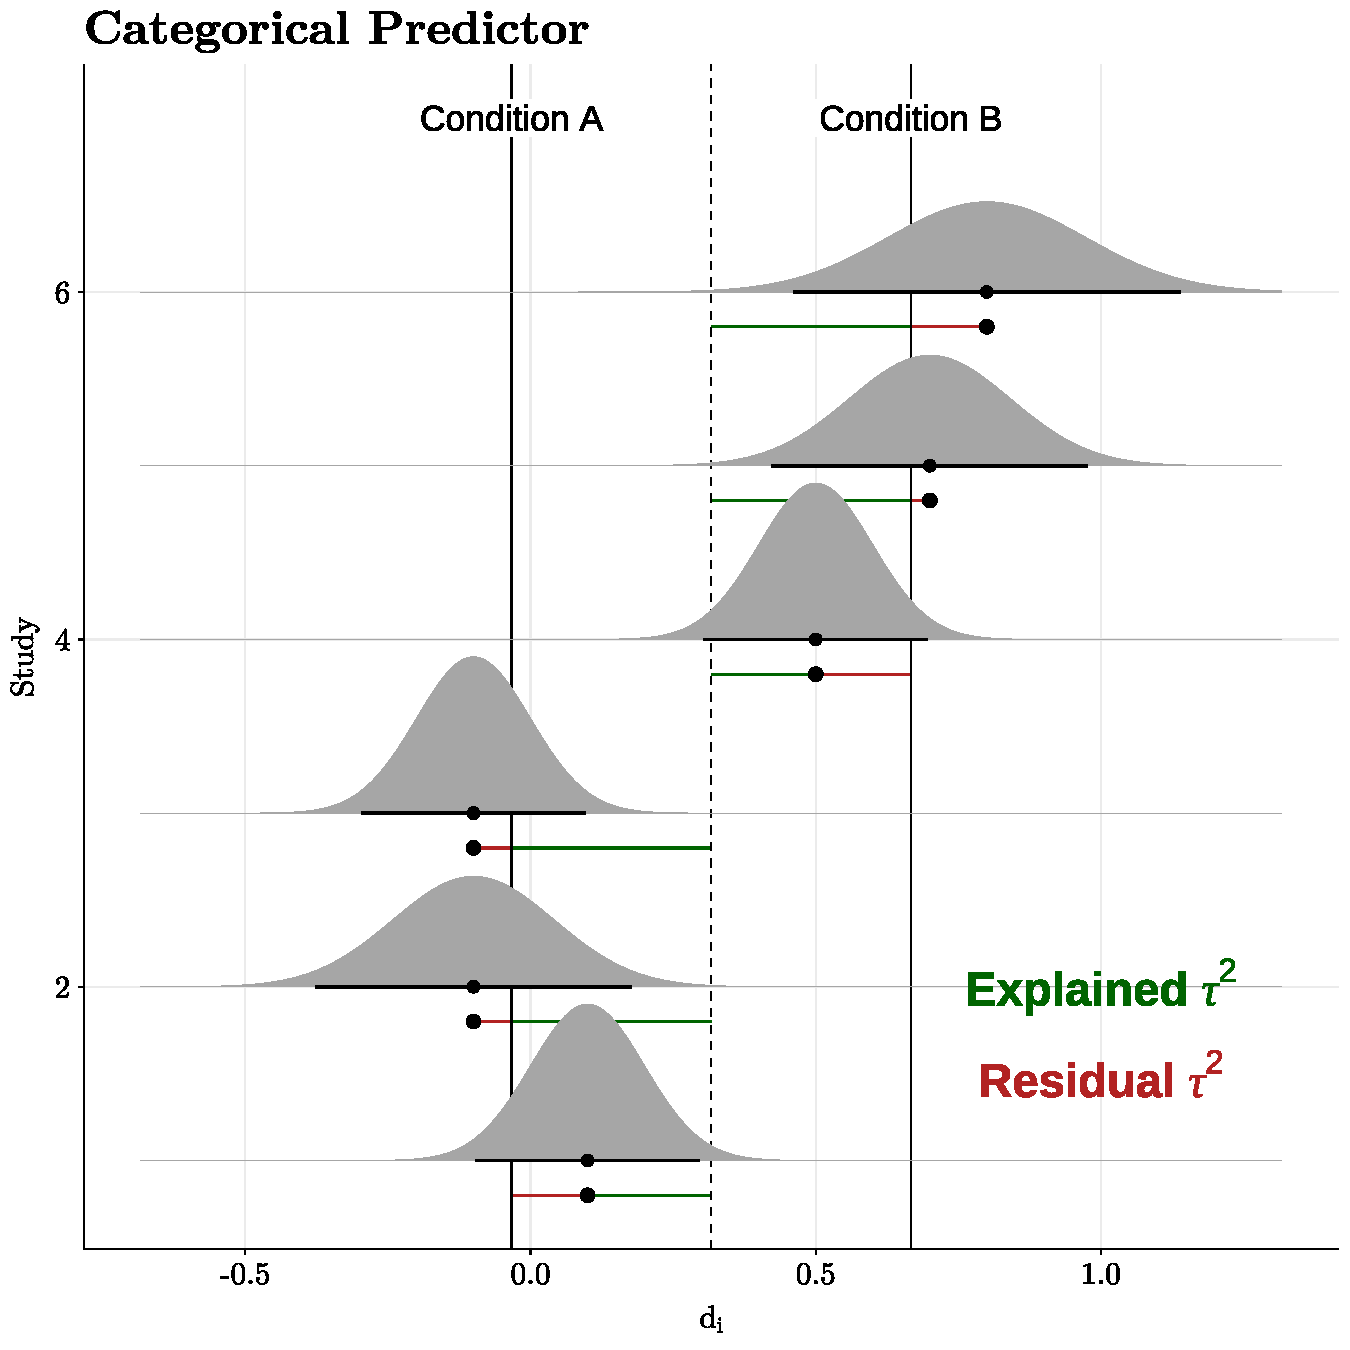
\includegraphics[width=0.8\linewidth]{C:/Users/user/Documents/work/shared-projects/simulating-meta-analysis/documents/output/paper_files/figure-latex/img-metaregression-bin-1} 

}

\caption{Graphical representation of a \emph{random-effects meta-regression} model with a categorical predictor (Condition A and Condition B). Each grey distribution represents the sampling distribution of included studies. The dotted line is the average effect (i.e., random-effects model without moderators). The effect size differs between conditions A and B, including the \emph{condition} moderator explaining part of the total heterogeneity (pink plus green segments). The green segments depict the explained heterogeneity, and the pink segments the residual (unexplained) heterogeneity. The pink squares are simulated observed effect sizes from the sampling distributions.}\label{fig:img-metaregression-bin}
\end{figure}

\normalsize

\scriptsize

\begin{figure}[H]

{\centering 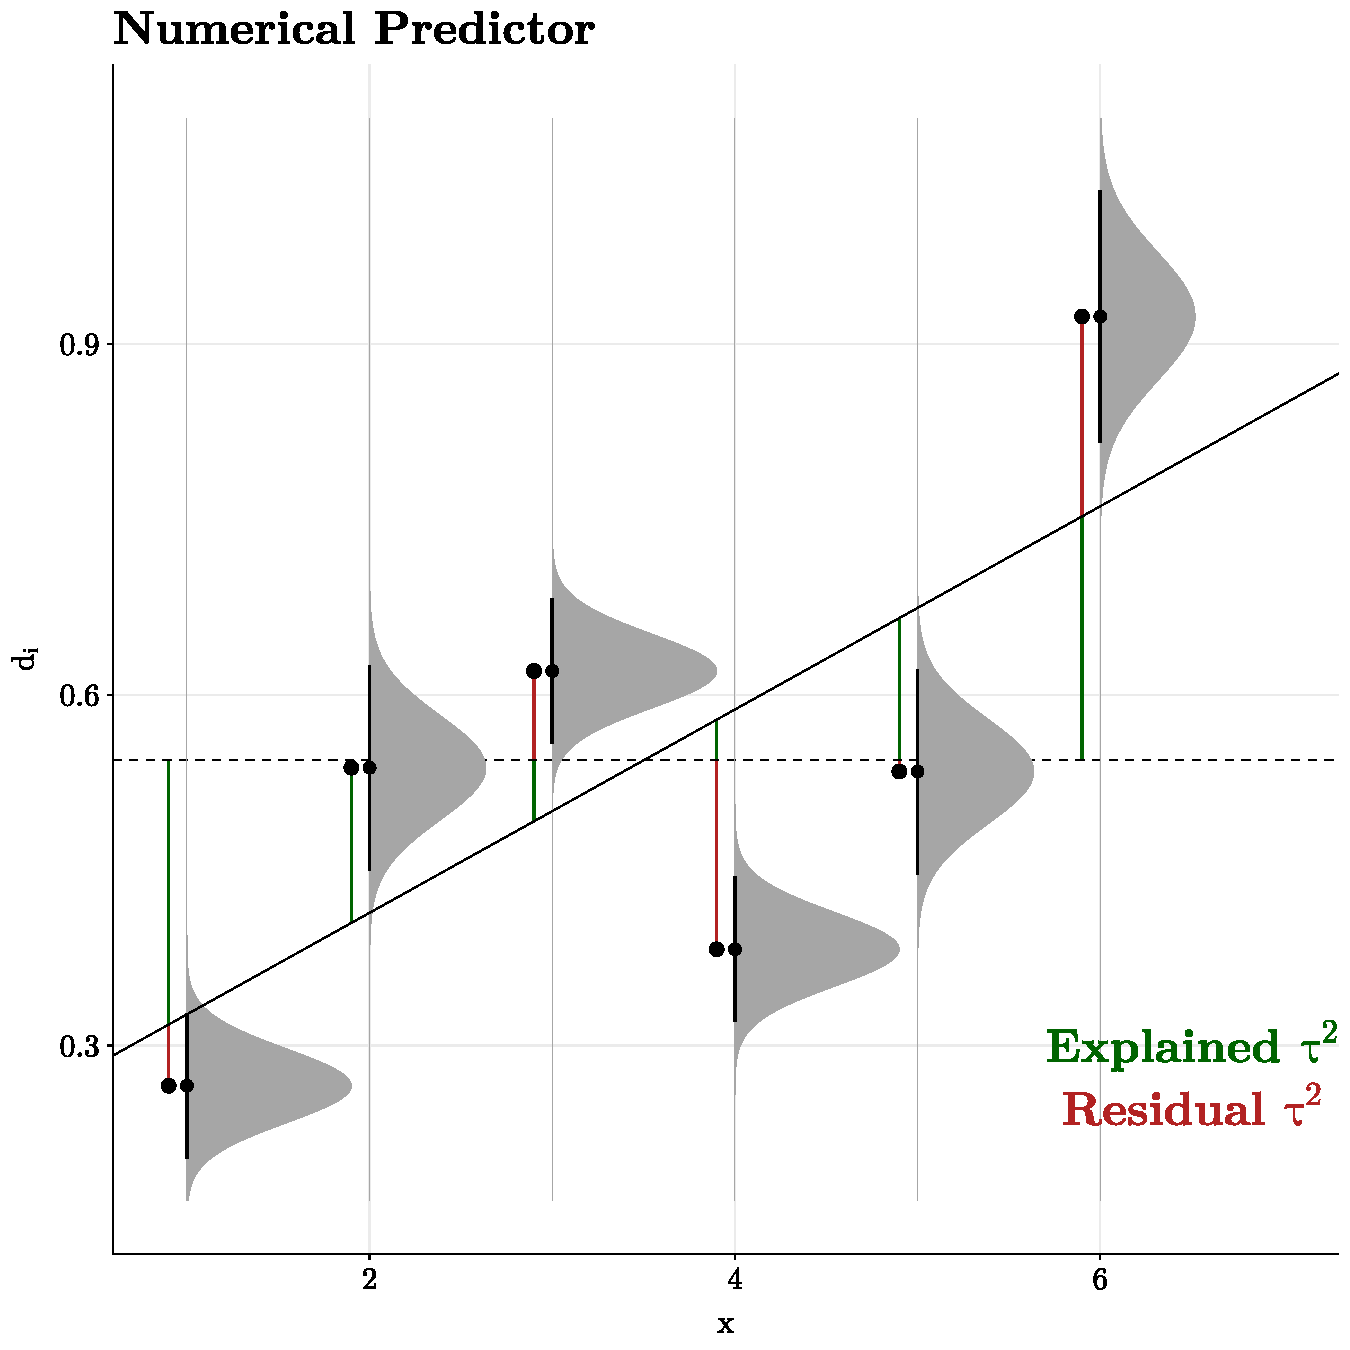
\includegraphics[width=0.8\linewidth]{C:/Users/user/Documents/work/shared-projects/simulating-meta-analysis/documents/output/paper_files/figure-latex/img-metaregression-num-1} 

}

\caption{Graphical representation of a \emph{random-effects meta-regression} model with a numerical predictor (\(x\)). Each grey distribution represents the sampling distribution of included studies. The dotted line is the average effect (i.e., random-effects model without moderators). The effect size increases as a function of the \(x\) variable. Therefore, including \(x\) as a predictor explains the
heterogeneity. The rest of the Figure follows the same logic as Figure \ref{fig:img-metaregression-bin}.}\label{fig:img-metaregression-num}
\end{figure}

\normalsize

\hypertarget{meta-regression-with-a-categorical-moderator}{%
\subsubsection{Meta-regression with a categorical moderator}\label{meta-regression-with-a-categorical-moderator}}

A common example of meta-regression is by including a categorical predictor, including information about study-level features. In our example, a group of studies uses an online memory task while others use a standard lab-based task. The Equation \eqref{eq:random-effects-model1} can be easily extended for a meta-regression model by including a variable encoding the type of task (online vs.~lab-based) and the expected difference between the two levels of the moderator (i.e., the \emph{lab vs.~online effect}). In regression terms (see equation \eqref{eq:meta-regression}), we could use a dummy variable (\(X_{1}\)) that takes the value of 0 for the \emph{lab-based task} (\emph{L}) and a value of 1 for an \emph{online task} (\emph{O})\footnote{The \emph{dummy coding} (also known as treatment coding) is the default in R and \texttt{metafor} but other coding schemes could be used (see Schad, Vasishth, Hohenstein, \& Kliegl, 2020 for an overview of contrast coding schemes). As in standard linear regression, the contrast coding of categorical factors or the presence/absence of the intercept influences the interpretation of estimated model parameters and omnibus meta-regression tests (see \url{https://www.metafor-project.org/doku.php/tips:models_with_or_without_intercept} for a detailed discussion)} . Now we fix \(\beta_{1}\) to be the \emph{lab vs.~online effect} (i.e., the expected mean difference between the two groups of studies) and the product between \(\beta_{1}X_{1_i}\) will consider the \emph{lab vs.~online effect}. Crucially, despite \(\tau^{2}\) is still the heterogeneity between effect sizes, now we need to fix \(\tau^{2}\) considering that we included a moderator. In other terms, \(\delta_i \sim \mathcal{N}(0, \tau_{r}^{2})\) where \(\tau^2_r\) is the residual heterogeneity after including the moderator. We can describe our model using equation \eqref{eq:meta-regression-equations} according to the value of \(X_{1_i}\) (L = lab-based experiments, O = online experiments).

\begin{align}
\begin{gathered}
y_i = \beta_0 + \delta_i + \beta_1 X_{1_i} + \epsilon_i
\label{eq:meta-regression}
\end{gathered}
\end{align}

\begin{align}
\begin{gathered}
y_{L_i} = \beta_0 + \delta_i + \beta_1 \times 0 + \epsilon_i \\
y_{O_i} = \beta_0 + \delta_i + \beta_1 \times 1 + \epsilon_i
\label{eq:meta-regression-equations}
\end{gathered}
\end{align}

We can simulate the same scenario of the random-effects model with \(k_O = 15\) (\emph{online tasks}) and \(k_L = 15\) (\emph{lab-based tasks}). Then we fix the \(\beta_1 = 0.2\) and \(\tau_r^2 = 0.1\) (\(r\) for residual).

\scriptsize

\begin{Shaded}
\begin{Highlighting}[]
\FunctionTok{set.seed}\NormalTok{(seed)}
\NormalTok{k }\OtherTok{\textless{}{-}} \DecValTok{30} \CommentTok{\# the total number of studies}
\NormalTok{b0 }\OtherTok{\textless{}{-}} \FloatTok{0.1} \CommentTok{\# intercept, the effect size of the lab{-}based studies}
\NormalTok{b1 }\OtherTok{\textless{}{-}} \FloatTok{0.2} \CommentTok{\# the difference between the two levels of the moderator}
\NormalTok{tau2r }\OtherTok{\textless{}{-}} \FloatTok{0.1} \CommentTok{\# the residual heterogeneity}
\NormalTok{n }\OtherTok{\textless{}{-}} \DecValTok{30} \CommentTok{\# the sample size per group, per study}

\NormalTok{sim }\OtherTok{\textless{}{-}} \FunctionTok{make\_data}\NormalTok{(}\AttributeTok{k =}\NormalTok{ k, }\AttributeTok{nc =}\NormalTok{ n, }\AttributeTok{nt =}\NormalTok{ n, }\AttributeTok{exp =} \FunctionTok{rep}\NormalTok{(}\FunctionTok{c}\NormalTok{(}\StringTok{"lab"}\NormalTok{, }\StringTok{"online"}\NormalTok{), }\AttributeTok{each =}\NormalTok{ k}\SpecialCharTok{/}\DecValTok{2}\NormalTok{))}

\NormalTok{sim}\SpecialCharTok{$}\NormalTok{deltai }\OtherTok{\textless{}{-}} \FunctionTok{rnorm}\NormalTok{(k, }\DecValTok{0}\NormalTok{, }\FunctionTok{sqrt}\NormalTok{(tau2r)) }\CommentTok{\# the by{-}study residual adjustment}
\NormalTok{sim}\SpecialCharTok{$}\NormalTok{es }\OtherTok{\textless{}{-}}\NormalTok{ b0 }\SpecialCharTok{+}\NormalTok{ sim}\SpecialCharTok{$}\NormalTok{deltai }\SpecialCharTok{+}\NormalTok{ b1}\SpecialCharTok{*}\FunctionTok{ifelse}\NormalTok{(sim}\SpecialCharTok{$}\NormalTok{exp }\SpecialCharTok{==} \StringTok{"lab"}\NormalTok{, }\DecValTok{0}\NormalTok{, }\DecValTok{1}\NormalTok{)}

\NormalTok{sim }\OtherTok{\textless{}{-}} \FunctionTok{sim\_studies}\NormalTok{(sim}\SpecialCharTok{$}\NormalTok{es, sim}\SpecialCharTok{$}\NormalTok{nc, sim}\SpecialCharTok{$}\NormalTok{nt, }\AttributeTok{data =}\NormalTok{ sim)}
\NormalTok{res }\OtherTok{\textless{}{-}} \FunctionTok{rma}\NormalTok{(yi, vi, }\AttributeTok{mods =} \SpecialCharTok{\textasciitilde{}}\NormalTok{exp, }\AttributeTok{method =} \StringTok{"REML"}\NormalTok{, }\AttributeTok{data =}\NormalTok{ sim)}
\end{Highlighting}
\end{Shaded}

\normalsize

Now we can fit the meta-regression model with the \texttt{rma} function as for the random-effects model with the addition of \texttt{mods\ =\ \textasciitilde{}\ exp} that indicates which variables to consider as moderators. The results are presented in Table \ref{tab:res-meta-reg-dummy}. Now the model will estimate an \emph{intercept} parameter (i.e., \(\beta_0\)) that is the value of \(y\) when \(X_1\) is zero (i.e., for lab-based studies) or in other terms the expected value for lab-based studies. Then the \(\beta_1\) parameter represents the estimated difference in \(y\) between the values of \(X_1\) (i.e., lab-based vs online experiments). As said before, \(\tau^2_r\) is now the residual heterogeneity that is interpreted as the variability between effect sizes after controlling for the moderator \(X_1\).

\scriptsize

\begin{table}[H]

\caption{\label{tab:res-meta-reg-dummy}Summary of the \emph{random-effect} model with a categorical predictor (lab vs online experiments). The \texttt{intercept} is the average effect for lab-based experiments and \texttt{exponline} is the difference between lab-based and online experiments. The \(R^2\) is the percentage of explained heterogeneity and \(\tau^2_r\) is the estimated residual heterogeneity. Other parameters are the same as the standard \emph{random-effect} model (see Table \ref{tab:res-random-effects}).}
\centering
\fontsize{9}{11}\selectfont
\begin{tabular}[t]{ccccc}
\toprule
 & $\beta$ & 95\% CI & z & p\\
\midrule
intercept & 0.038 (SE = 0.101) & $[-0.161, 0.236]$ & 0.372 & 0.710\\
exponline & 0.323 (SE = 0.143) & $[0.043, 0.602]$ & 2.263 & 0.024\\
\bottomrule
\multicolumn{5}{l}{\textsuperscript{} $k = 30$}\\
\multicolumn{5}{l}{\textsuperscript{} $\tau^2_r = 0.087$ ($SE = 0.041$)}\\
\multicolumn{5}{l}{\textsuperscript{} $R^2 = 20.659\%$}\\
\multicolumn{5}{l}{\textsuperscript{} $I^2 = 57.741\%$}\\
\end{tabular}
\end{table}

\normalsize

\hypertarget{meta-regression-with-a-numerical-moderator}{%
\subsubsection{Meta-regression with a numerical moderator}\label{meta-regression-with-a-numerical-moderator}}

The same approach can be used for a continuous predictor. For example, we can simulate that the average participant's age within each study could explain part of the observed heterogeneity. Now the \(X_1\) is a continuous predictor representing the average age for each study and \(\beta_1\) is the effect size increase for a unit increase (i.e., 1 year) of average age. Sometimes guessing a plausible \(\beta_1\) value with a continuous predictor is not straightforward. A first strategy could be to use values estimated from the literature. Another approach consists in setting up the model and simulating several expected \(y_i\) and calculating the range of simulated values. A third possibility is fixing the proportion of explained heterogeneity calculating the \(\beta_1\) value accordingly. As in standard regression analysis, we can use the \(R^2\) statistic to describe the amount of heterogeneity explained by the included moderators. Equation \eqref{eq:rsquared} reports how to calculate the \(R^2\) for a meta-regression model. The \(\tau^2_{r}\) is the residual heterogeneity after considering the moderators and \(\tau^2_{f}\) is the heterogeneity estimated without considering the moderators. In the next sections, we will present an example of the simulation-based and the \(R^2\) based approaches.

\begin{align}
\begin{aligned}
R^2 = 1 - \frac{\tau^2_{r}}{\tau^2_{f}}
\label{eq:rsquared}
\end{aligned}
\end{align}

In terms of regression parameters now the intercept (\(\beta_0\)) is no longer the overall effect or the average of one category as in the previous example but the estimated value for a specific \(X_1\) thus for a specific age. If \(X_1\) is a variable representing the average age for each study, then the \(\beta_0\) is the average effect size when the age is zero. Depending on the moderator, the intercept is interpreted in different ways. For example, with the age, the intercept has no empirical meaning given that no studies could have a participant average age of zero. A strategy could be to mean-center the age (i.e., subtracting from each study age the average age across the study). Now the intercept is still the average effect size when the age is zero but now zero is the average age. Importantly, the contrast coding for categorical predictors or centering numerical variables does not affect the overall model but only parameters values and interpretation.

\hypertarget{assessing-the-impact-of-beta_1}{%
\paragraph{\texorpdfstring{Assessing the impact of \(\beta_1\)}{Assessing the impact of \textbackslash beta\_1}}\label{assessing-the-impact-of-beta_1}}

As reported in the previous section, a strategy to guess plausible values for \(\beta_{1}\) is by simulating several expected \(y_{i}\) given the meta-regression equation and summarizing or plotting the effect size range. The range of simulated \(y_{i}\) values are also affected by the simulated age values across studies. However, it is probably more intuitive to guess a plausible range of moderator values compared to the \(\beta_{1}\) value. In this specific example, if all studies target a specific population (e.g., adults below 50 years), the expected average age range can be easily simulated. In our case, we simulated \(k\) average age values from a uniform distribution \(\text{age}_{i} \sim U\left( 20,40 \right)\). Then we can plot the distribution of \(y_{i}\) values to check the plausibility of simulated values. As shown in Figure \ref{fig:plot-meta-reg-plausible-implausible}, with the same range for the moderator, a \(\beta_{1} = 0.1\) gives a plausible effect sizes range while a \(\beta_{1} = 0.7\) predicts very extreme values.

\scriptsize

\begin{Shaded}
\begin{Highlighting}[]
\FunctionTok{set.seed}\NormalTok{(seed)}
\NormalTok{k }\OtherTok{\textless{}{-}} \DecValTok{1000} \CommentTok{\# number of studies}
\NormalTok{b0 }\OtherTok{\textless{}{-}} \FloatTok{0.3} \CommentTok{\# the intercept i.e., average yi when x is 0}
\NormalTok{b1 }\OtherTok{\textless{}{-}} \FunctionTok{c}\NormalTok{(}\FloatTok{0.1}\NormalTok{, }\FloatTok{0.7}\NormalTok{) }\CommentTok{\# the beta1 i.e., the increase in yi for an increase in 1 year}
\NormalTok{tau2r }\OtherTok{\textless{}{-}} \FloatTok{0.1} \CommentTok{\# the residual heterogeneity after including x1}
\NormalTok{n }\OtherTok{\textless{}{-}} \DecValTok{30} \CommentTok{\# number of participants per study, per group}
\NormalTok{x1 }\OtherTok{\textless{}{-}} \FunctionTok{runif}\NormalTok{(k, }\DecValTok{20}\NormalTok{, }\DecValTok{40}\NormalTok{) }\CommentTok{\# random mean{-}age for each study}
\NormalTok{x10 }\OtherTok{\textless{}{-}}\NormalTok{ x1 }\SpecialCharTok{{-}} \FunctionTok{mean}\NormalTok{(x1) }\CommentTok{\# centering the age}

\NormalTok{sim }\OtherTok{\textless{}{-}}\NormalTok{ tidyr}\SpecialCharTok{::}\FunctionTok{expand\_grid}\NormalTok{(}\AttributeTok{id =} \DecValTok{1}\SpecialCharTok{:}\NormalTok{k, }\AttributeTok{nc =}\NormalTok{ n, }\AttributeTok{nt =}\NormalTok{ n, }\AttributeTok{b1 =}\NormalTok{ b1)}

\NormalTok{sim}\SpecialCharTok{$}\NormalTok{age }\OtherTok{\textless{}{-}} \FunctionTok{rep}\NormalTok{(x1, }\AttributeTok{each =} \DecValTok{2}\NormalTok{)}
\NormalTok{sim}\SpecialCharTok{$}\NormalTok{age0 }\OtherTok{\textless{}{-}} \FunctionTok{rep}\NormalTok{(x10, }\AttributeTok{each =} \DecValTok{2}\NormalTok{)}

\NormalTok{deltai }\OtherTok{\textless{}{-}} \FunctionTok{rnorm}\NormalTok{(k, }\DecValTok{0}\NormalTok{, }\FunctionTok{sqrt}\NormalTok{(tau2r))}
\NormalTok{sim}\SpecialCharTok{$}\NormalTok{deltai }\OtherTok{\textless{}{-}} \FunctionTok{rep}\NormalTok{(deltai, }\AttributeTok{each =} \DecValTok{2}\NormalTok{)}

\NormalTok{sim}\SpecialCharTok{$}\NormalTok{es }\OtherTok{\textless{}{-}}\NormalTok{ b0 }\SpecialCharTok{+}\NormalTok{ sim}\SpecialCharTok{$}\NormalTok{deltai }\SpecialCharTok{+}\NormalTok{ sim}\SpecialCharTok{$}\NormalTok{b1}\SpecialCharTok{*}\NormalTok{sim}\SpecialCharTok{$}\NormalTok{age0}

\NormalTok{sim }\OtherTok{\textless{}{-}} \FunctionTok{sim\_studies}\NormalTok{(sim}\SpecialCharTok{$}\NormalTok{es, sim}\SpecialCharTok{$}\NormalTok{nc, sim}\SpecialCharTok{$}\NormalTok{nt, }\AttributeTok{data =}\NormalTok{ sim)}
\end{Highlighting}
\end{Shaded}

\normalsize

\scriptsize

\begin{figure}[H]

{\centering 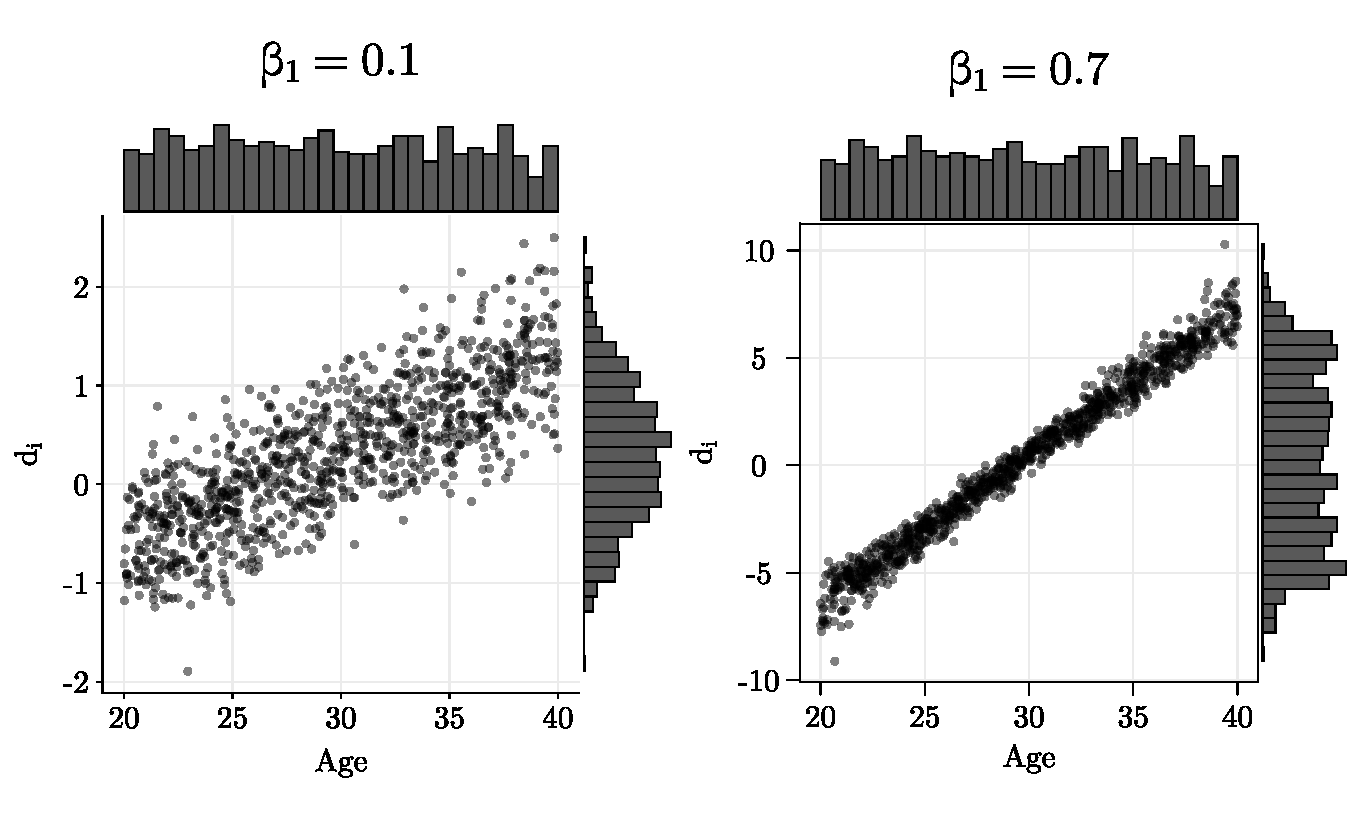
\includegraphics[width=0.8\linewidth]{C:/Users/user/Documents/work/shared-projects/simulating-meta-analysis/documents/output/paper_files/figure-latex/plot-meta-reg-plausible-implausible-1} 

}

\caption{Scatter plots with marginal histograms for the range of simulated \(y_i\) with two \(\beta_1\) values. The x-axis depicts the average age of simulated studies and the y-axis depicts the simulated effect size. On the left, the majority of simulated values range between -1.5 and 1.5 thus \(\beta_1 = 0.1\) can be considered a plausible value. On the right, (\(\beta = 0.7\)) values range between -10 to 10 that despite theoretically possible can be considered highly implausible values in real meta-analyses for psychological data.}\label{fig:plot-meta-reg-plausible-implausible}
\end{figure}

\normalsize

\hypertarget{simulating-using-r2}{%
\paragraph{\texorpdfstring{Simulating using \(R^2\)}{Simulating using R\^{}2}}\label{simulating-using-r2}}

A more intuitive way to simulate a continuous predictor is fixing the desired \(R^{2}\) value and finding the coefficient that produces the desired value. This approach has been implemented by Lopez-Lopez and colleagues (2014). We can use Equation \eqref{eq:beta-from-r21} and \eqref{eq:beta-from-r22} to find the \(\beta_{1}\) value that is associated with a certain \(R^{2}\).

\begin{align}
\begin{aligned}
\beta^2_1 = \tau^2R^2
\label{eq:beta-from-r21}
\end{aligned}
\end{align}

\begin{align}
\begin{aligned}
\tau^2_{r} = \tau^2 - \beta^2_1
\label{eq:beta-from-r22}
\end{aligned}
\end{align}

Now we can simulate the regression model using \(\sqrt{\beta^2_1}\) as coefficient and \(\tau_{r}^{2}\) as residual heterogeneity. Results from the fitted model fixing the \(R^{2}\) values are presented in Table \ref{tab:res-meta-reg-numerical-r2} and Figure \ref{fig:plot-meta-reg-numerical-r2}. As Lopez-Lopez and colleagues (2014) demonstrated, to reliably estimate \(R^{2}\) the number of studies needs to be large\footnote{see also \url{https://www.metafor-project.org/doku.php/tips:ci_for_r2} for a discussion about confidence intervals for the \(R^2\) statistic}. Lopez-Lopez and colleagues (2014) generated the moderator (\(X_{1}\)) values from a standard normal distribution. In the following example, we standardized the moderator (\texttt{scale()}) after simulating values on the \emph{age} scale (e.g., \texttt{runif(k,\ 20,\ 40)}).

\scriptsize

\begin{Shaded}
\begin{Highlighting}[]
\FunctionTok{set.seed}\NormalTok{(seed)}
\NormalTok{k }\OtherTok{\textless{}{-}} \DecValTok{100} \CommentTok{\# the number of studies}
\NormalTok{r2 }\OtherTok{\textless{}{-}} \FloatTok{0.2} \CommentTok{\# the desired r2 value}
\NormalTok{tau2 }\OtherTok{\textless{}{-}} \FloatTok{0.3} \CommentTok{\# the overall tau2}
\NormalTok{b0 }\OtherTok{\textless{}{-}} \FloatTok{0.3} \CommentTok{\# the intercept i.e., average yi when x1 is 0}
\NormalTok{b1\_2 }\OtherTok{\textless{}{-}}\NormalTok{ tau2 }\SpecialCharTok{*}\NormalTok{ r2 }\CommentTok{\# the beta1\^{}2 i.e., the increase in yi for an increase in 1 year}
\NormalTok{b1 }\OtherTok{\textless{}{-}} \FunctionTok{sqrt}\NormalTok{(b1\_2) }\CommentTok{\# b1\_2 is squared, back to the original scale}
\NormalTok{tau2r }\OtherTok{\textless{}{-}}\NormalTok{ tau2 }\SpecialCharTok{{-}}\NormalTok{ b1\_2 }\CommentTok{\# the residual heterogeneity after including x1}
\NormalTok{n }\OtherTok{\textless{}{-}} \DecValTok{30} \CommentTok{\# number of participants per study, per group}
\NormalTok{x1 }\OtherTok{\textless{}{-}} \FunctionTok{runif}\NormalTok{(k, }\DecValTok{20}\NormalTok{, }\DecValTok{40}\NormalTok{) }\CommentTok{\# random mean{-}age for each study}

\NormalTok{sim }\OtherTok{\textless{}{-}} \FunctionTok{make\_data}\NormalTok{(}\AttributeTok{k =}\NormalTok{ k, }\AttributeTok{nt =}\NormalTok{ n, }\AttributeTok{nc =}\NormalTok{ n, }\AttributeTok{age =}\NormalTok{ x1)}

\NormalTok{sim}\SpecialCharTok{$}\NormalTok{deltai }\OtherTok{\textless{}{-}} \FunctionTok{rnorm}\NormalTok{(k, }\DecValTok{0}\NormalTok{, }\FunctionTok{sqrt}\NormalTok{(tau2r))}
\NormalTok{sim}\SpecialCharTok{$}\NormalTok{age0 }\OtherTok{\textless{}{-}} \FunctionTok{scale}\NormalTok{(sim}\SpecialCharTok{$}\NormalTok{age, }\AttributeTok{center =} \ConstantTok{TRUE}\NormalTok{, }\AttributeTok{scale =} \ConstantTok{TRUE}\NormalTok{) }\CommentTok{\# standardize the moderator}
\NormalTok{sim}\SpecialCharTok{$}\NormalTok{es }\OtherTok{\textless{}{-}}\NormalTok{ b0 }\SpecialCharTok{+}\NormalTok{ sim}\SpecialCharTok{$}\NormalTok{deltai }\SpecialCharTok{+}\NormalTok{ b1}\SpecialCharTok{*}\NormalTok{sim}\SpecialCharTok{$}\NormalTok{age0}

\NormalTok{sim }\OtherTok{\textless{}{-}} \FunctionTok{sim\_studies}\NormalTok{(sim}\SpecialCharTok{$}\NormalTok{es, sim}\SpecialCharTok{$}\NormalTok{nt, sim}\SpecialCharTok{$}\NormalTok{nc, }\AttributeTok{data =}\NormalTok{ sim)}
\NormalTok{res }\OtherTok{\textless{}{-}} \FunctionTok{rma}\NormalTok{(yi, vi, }\AttributeTok{mods =} \SpecialCharTok{\textasciitilde{}}\NormalTok{age0, }\AttributeTok{method =} \StringTok{"REML"}\NormalTok{, }\AttributeTok{data =}\NormalTok{ sim)}
\end{Highlighting}
\end{Shaded}

\normalsize

\scriptsize

\begin{table}[H]

\caption{\label{tab:res-meta-reg-numerical-r2}Summary of the \emph{random-effects} model fixing the \(R^{2}\) value. The \texttt{intercept} is the effect size for the average \texttt{age} (given that age is mean-centered). The \texttt{age0} parameter is the slope between \texttt{age} and the effect size interpreted as an increase in effect size for a unit increase in the average age. Other parameters are the same as described in Table \ref{tab:res-random-effects} and \ref{tab:res-meta-reg-dummy}.}
\centering
\fontsize{9}{11}\selectfont
\begin{tabular}[t]{ccccc}
\toprule
 & $\beta$ & 95\% CI & z & p\\
\midrule
intercept & 0.339 (SE = 0.051) & $[0.239, 0.439]$ & 6.643 & < 0.001\\
age0 & 0.168 (SE = 0.051) & $[0.067, 0.268]$ & 3.272 & 0.001\\
\bottomrule
\multicolumn{5}{l}{\textsuperscript{} $k = 100$}\\
\multicolumn{5}{l}{\textsuperscript{} $\tau^2_r = 0.197$ ($SE = 0.037$)}\\
\multicolumn{5}{l}{\textsuperscript{} $R^2 = 11.029\%$}\\
\multicolumn{5}{l}{\textsuperscript{} $I^2 = 76.611\%$}\\
\end{tabular}
\end{table}

\normalsize

\scriptsize

\begin{figure}[H]

{\centering 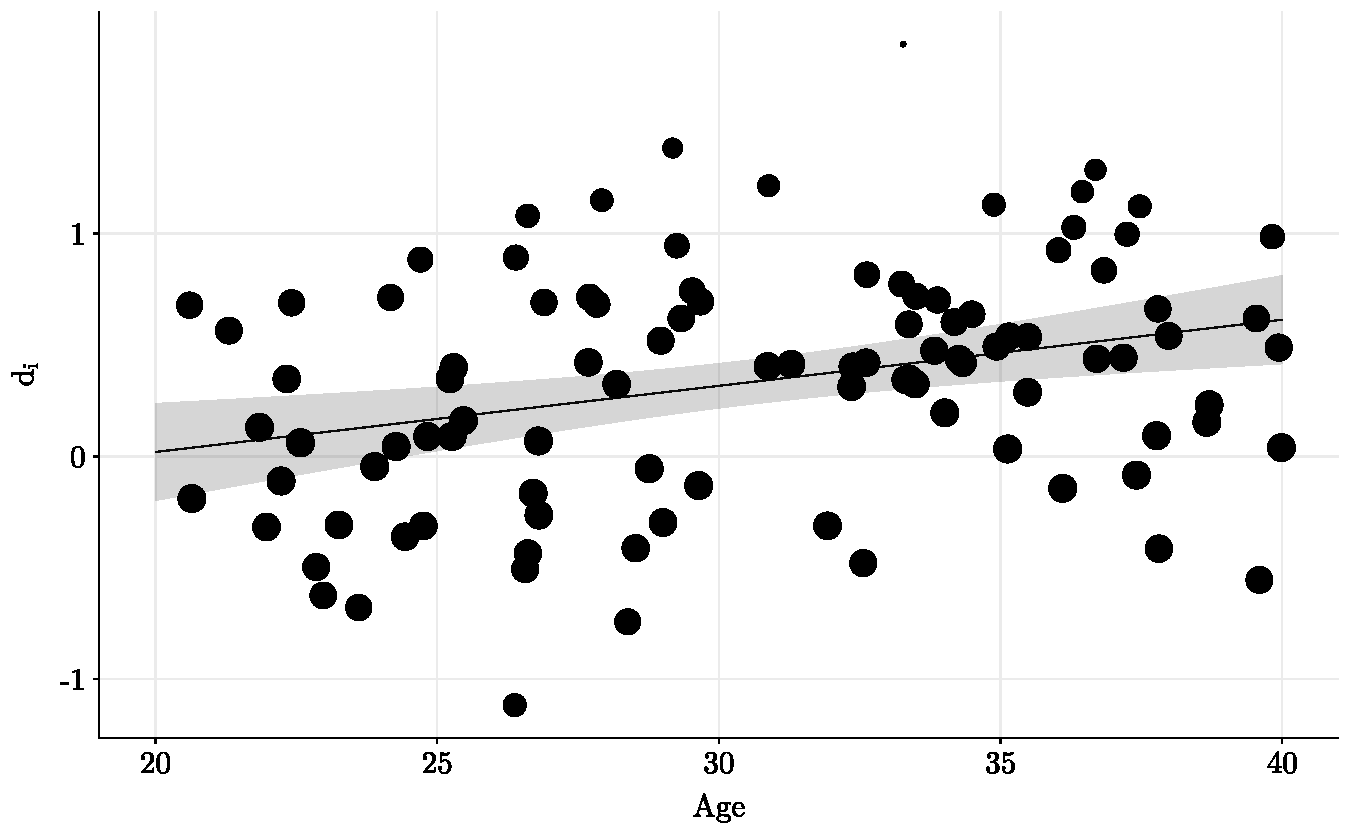
\includegraphics[width=0.8\linewidth]{C:/Users/user/Documents/work/shared-projects/simulating-meta-analysis/documents/output/paper_files/figure-latex/plot-meta-reg-numerical-r2-1} 

}

\caption{Meta-regression results for the \emph{random-effects model} with a numerical moderator. Each effect size is represented with a black dot where the dimension represents the weight according to the inverse of the variance. The line represents the estimated meta-regression slope with the 95\% confidence interval (grey bands).}\label{fig:plot-meta-reg-numerical-r2}
\end{figure}

\normalsize

\hypertarget{power-analysis}{%
\section{Power Analysis}\label{power-analysis}}

The previous simulation examples can be easily implemented for multiple purposes. For example, we can use different effect sizes and variance estimators when using the \texttt{sim\_study()} function to check the impact on the fitted meta-analysis model. However, one of the most critical applications is estimating the power of a specific statistical model. One of the purposes of power analysis by simulations is to estimate the required number of studies to detect an hypothetical effect size when planning a meta-analysis. At the same time, the meta-analysis that we presented (\emph{two-level} equal or random-effects model) can be considered as a multi-lab (e.g., Klein et al., 2018) study where experiments are planned and not collected from the literature. We can use the same simulation approach to optimize the number of participants and studies when planning a multi-lab project.

As explained in the introduction, there are several approaches and tools to estimate the power of \emph{equal} and \emph{random-effects models} (see Borenstein et al., 2009, Chapter 29; Harrer et al., 2019, Chapter 14). These methods are easy to implement but made strong assumptions, such as the homogeneity of sample size, and did not consider the uncertainty in estimating \(\tau^{2}\). Jackson and colleagues (2017) partially solve the issue by developing an interesting method that takes into account the uncertainty in estimating \(\tau^{2}\) without using simulations. However, complex simulation scenarios can be handled only using Monte Carlo methods.

A general Monte Carlo simulation for the power analysis can be implemented with the following steps:

\begin{enumerate}
\def\labelenumi{\arabic{enumi}.}
\tightlist
\item
  Choose the model that generates the data (e.g., equal or random-effects model).
\item
  Fix the relevant parameters (e.g., \(\tau^{2}\) and \(\theta\)).
\item
  Simulate a dataset.
\item
  Fit the appropriate model.
\item
  Store the p-value associated with the parameter of interest
\item
  Repeat 3-5 a large number of times (e.g., 10000).
\item
  Calculate the power as the proportion of p-values below the \(\alpha\) level.
\end{enumerate}

For example, we can estimate the power of a \emph{random-effects} model by repeating the simulation presented in Section \ref{re-model} many times. We simulated heterogeneity of sample sizes sampling \(n_{T}\) and \(n_{C}\) values from a Poisson distribution with \(\lambda = 20\). In this way, on average, the sample size is 20 for primary studies with a certain amount of heterogeneity. Usually, it is more informative to simulate different scenarios according to the relevant parameters, such as sample sizes, number of studies, or heterogeneity. For example, we can estimate the power with a different number of studies \(k\). We define the \texttt{do\_sim()} function that, according to the input parameter, repeats the simulation a certain number of times (i.e., \texttt{nsim})\footnote{We are using the \texttt{purrr::pmap()} function that can be considered very similar to \texttt{mapply()} but less verbose. Compared to \texttt{mapply()}, the \texttt{sim\_grid} columns are directly passed to the \texttt{do\_sim()} function without specifying the order.}. Increasing the number of simulations will increase the power analysis estimation precision. Then the \texttt{summary\_sim()} function analyzes each simulation returning the relevant values. We repeat the simulation of the \emph{random-effects} model several times with different parameters.

\scriptsize

\begin{Shaded}
\begin{Highlighting}[]

\NormalTok{do\_sim }\OtherTok{\textless{}{-}} \ControlFlowTok{function}\NormalTok{(k, mu, tau2, navg, nmin, nsim, }\AttributeTok{alpha =} \FloatTok{0.05}\NormalTok{, }\AttributeTok{summary =} \ConstantTok{TRUE}\NormalTok{)\{}
  \CommentTok{\# preallocate for computation speed}
\NormalTok{  p }\OtherTok{\textless{}{-}} \FunctionTok{vector}\NormalTok{(}\AttributeTok{mode =} \StringTok{"numeric"}\NormalTok{, }\AttributeTok{length =}\NormalTok{ nsim)}
  
  \CommentTok{\# start the simulation loop}
  \ControlFlowTok{for}\NormalTok{(i }\ControlFlowTok{in} \DecValTok{1}\SpecialCharTok{:}\NormalTok{nsim)\{}
\NormalTok{    deltai }\OtherTok{\textless{}{-}} \FunctionTok{rnorm}\NormalTok{(k, }\DecValTok{0}\NormalTok{, }\FunctionTok{sqrt}\NormalTok{(tau2))}
\NormalTok{    es }\OtherTok{\textless{}{-}}\NormalTok{ mu }\SpecialCharTok{+}\NormalTok{ deltai}
    \CommentTok{\# simulate sample size, it is possible to use other distributions e.g., Gaussian}
\NormalTok{    n }\OtherTok{\textless{}{-}}\NormalTok{ nmin }\SpecialCharTok{+} \FunctionTok{rpois}\NormalTok{(k, navg }\SpecialCharTok{{-}}\NormalTok{ nmin)}
    \CommentTok{\# simulate the studies}
\NormalTok{    sim }\OtherTok{\textless{}{-}} \FunctionTok{sim\_studies}\NormalTok{(es, n, n, }\AttributeTok{data =} \ConstantTok{NULL}\NormalTok{)}
\NormalTok{    res }\OtherTok{\textless{}{-}} \FunctionTok{rma}\NormalTok{(yi, vi, }\AttributeTok{method =} \StringTok{"REML"}\NormalTok{, }\AttributeTok{data =}\NormalTok{ sim)}
\NormalTok{    p[i] }\OtherTok{\textless{}{-}}\NormalTok{ res}\SpecialCharTok{$}\NormalTok{pval }\CommentTok{\# store the p value}
\NormalTok{  \}}
  \ControlFlowTok{if}\NormalTok{(summary)\{}
    \CommentTok{\# return directly the power}
    \FunctionTok{summary\_sim}\NormalTok{(p, alpha)}
\NormalTok{  \}}\ControlFlowTok{else}\NormalTok{\{}
    \CommentTok{\# return the list of pvalues}
    \FunctionTok{data.frame}\NormalTok{(p)}
\NormalTok{  \}}
\NormalTok{\}}

\NormalTok{summary\_sim }\OtherTok{\textless{}{-}} \ControlFlowTok{function}\NormalTok{(p, alpha)\{}
\NormalTok{  power }\OtherTok{\textless{}{-}} \FunctionTok{mean}\NormalTok{(p }\SpecialCharTok{\textless{}=}\NormalTok{ alpha) }\CommentTok{\# compute power}
  \FunctionTok{data.frame}\NormalTok{(power)}
\NormalTok{\}}
\end{Highlighting}
\end{Shaded}

\normalsize

Simulation results are presented in Figure \ref{fig:plot-power-analysis} and Table \ref{tab:tab-power-analysis-example} showing that to reach 80\% power (usually considered an appropriate level) with \(\alpha = 0.05\) we need \textasciitilde35 studies. The same approach could be used to estimate the power of a meta-regression by simply modifying the \texttt{do\_sim()} function simulating the effect of a moderator and extracting the relevant p-value.

\scriptsize

\begin{Shaded}
\begin{Highlighting}[]
\FunctionTok{set.seed}\NormalTok{(seed)}
\NormalTok{nsim }\OtherTok{\textless{}{-}} \DecValTok{5000} \CommentTok{\# number of simulations per condition (5000, higher is better)}
\NormalTok{k }\OtherTok{\textless{}{-}} \FunctionTok{c}\NormalTok{(}\DecValTok{5}\NormalTok{, }\DecValTok{15}\NormalTok{, }\DecValTok{25}\NormalTok{, }\DecValTok{35}\NormalTok{, }\DecValTok{50}\NormalTok{) }\CommentTok{\# number of studies}
\NormalTok{delta }\OtherTok{\textless{}{-}} \FloatTok{0.3} \CommentTok{\# the average effect size}
\NormalTok{tau2 }\OtherTok{\textless{}{-}} \FloatTok{0.3} \CommentTok{\# the heterogeneity}
\NormalTok{navg }\OtherTok{\textless{}{-}} \DecValTok{20} \CommentTok{\# average sample size per study}
\NormalTok{nmin }\OtherTok{\textless{}{-}} \DecValTok{10} \CommentTok{\# minimum sample size per study}
\NormalTok{alpha }\OtherTok{\textless{}{-}} \FloatTok{0.05} \CommentTok{\# the alpha level}

\CommentTok{\# creating all combinations}
\NormalTok{sim\_grid }\OtherTok{\textless{}{-}}\NormalTok{ tidyr}\SpecialCharTok{::}\FunctionTok{expand\_grid}\NormalTok{(k, }\AttributeTok{mu =}\NormalTok{ delta, tau2, navg, nmin, nsim)}

\CommentTok{\# apply the simulation to all combinations}
\NormalTok{res }\OtherTok{\textless{}{-}}\NormalTok{ purrr}\SpecialCharTok{::}\FunctionTok{pmap}\NormalTok{(sim\_grid, do\_sim)}

\CommentTok{\# combine the results}
\NormalTok{res }\OtherTok{\textless{}{-}}\NormalTok{ dplyr}\SpecialCharTok{::}\FunctionTok{bind\_rows}\NormalTok{(res)}
\NormalTok{sim\_grid }\OtherTok{\textless{}{-}} \FunctionTok{cbind}\NormalTok{(sim\_grid, res)}
\end{Highlighting}
\end{Shaded}

\normalsize

\scriptsize

\begin{table}[H]

\begin{center}
\begin{threeparttable}

\caption{\label{tab:tab-power-analysis-example}The results from the power analysis simulation. The table depicts the simulation parameters, the estimated power using the \texttt{summary\_sim()} function, and the average sample size (\(n\)) across the simulations.}

\small{

\begin{tabular}{lllllll}
\toprule
k & \multicolumn{1}{c}{$\Delta$} & \multicolumn{1}{c}{$\tau^2$} & \multicolumn{1}{c}{$n_{avg}$} & \multicolumn{1}{c}{$n_{min}$} & \multicolumn{1}{c}{nsim} & \multicolumn{1}{c}{Power}\\
\midrule
5 & 0.30 & 0.30 & 20 & 10 & 5000 & 0.26\\
15 & 0.30 & 0.30 & 20 & 10 & 5000 & 0.47\\
25 & 0.30 & 0.30 & 20 & 10 & 5000 & 0.65\\
35 & 0.30 & 0.30 & 20 & 10 & 5000 & 0.79\\
50 & 0.30 & 0.30 & 20 & 10 & 5000 & 0.92\\
\bottomrule
\end{tabular}

}

\end{threeparttable}
\end{center}

\end{table}

\normalsize

\scriptsize

\begin{figure}[H]

{\centering 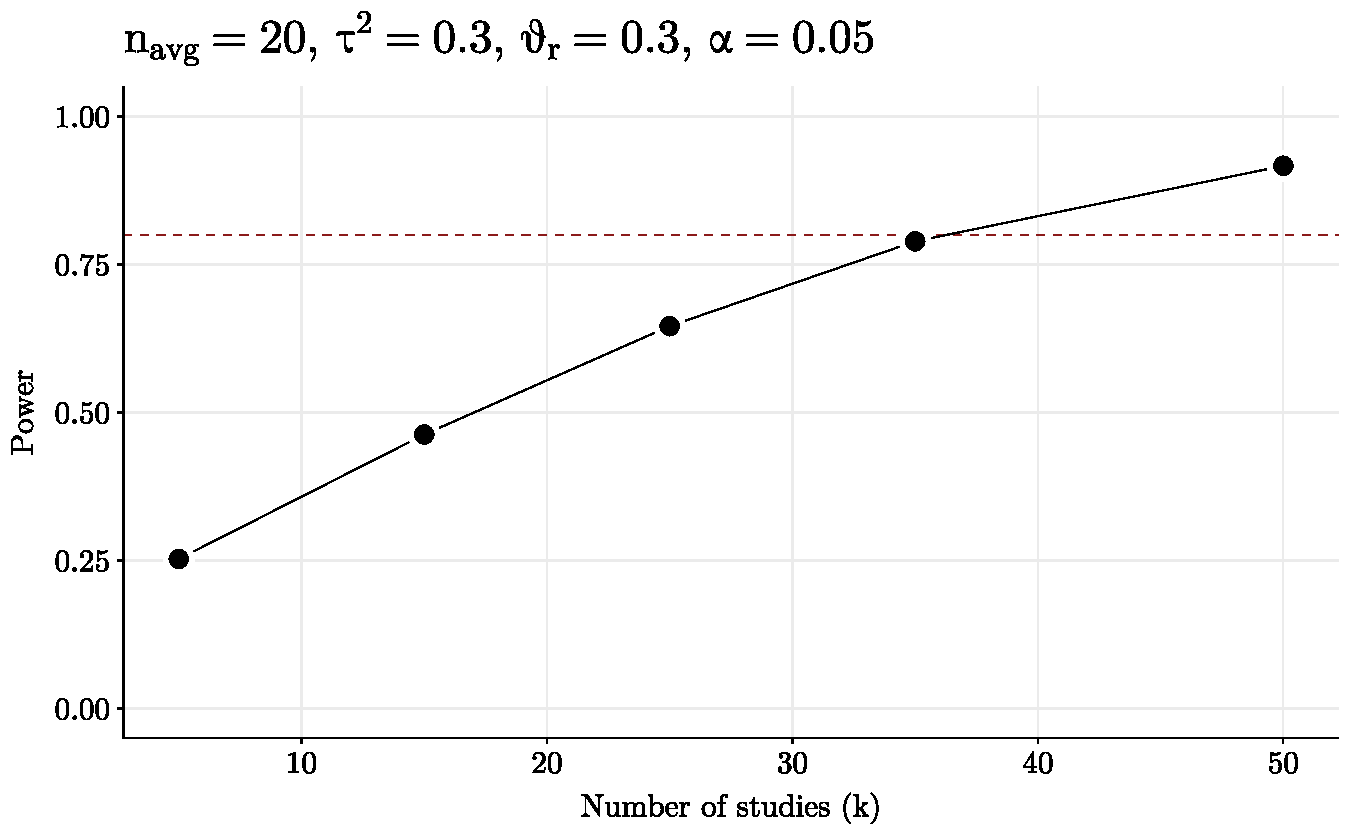
\includegraphics[width=0.8\linewidth]{C:/Users/user/Documents/work/shared-projects/simulating-meta-analysis/documents/output/paper_files/figure-latex/plot-power-analysis-1} 

}

\caption{Results from the \emph{random-effects model} power analysis. The x-axis depicts the number of studies (\(k\)), and the y-axis the estimated power. The pink dotted line is the 80\% power level, usually considered a good value for power analysis.}\label{fig:plot-power-analysis}
\end{figure}

\normalsize

\hypertarget{conclusions}{%
\section{Conclusions}\label{conclusions}}

The present work introduced the basic concepts of the meta-analysis regarding equal-effects, random-effects and meta-regression models with a simulation-based approach. We believe the presented examples are useful to implement alternative or more complex models. For example, the \texttt{sim\_study()} function can be easily modified to simulate another effect sizes index, such as correlations or odds ratios. In addition, more complex models, such as \emph{multivariate} or \emph{multilevel} models, can be simulated following a similar approach (see the supplementary materials). The \emph{multilevel} (e.g., \emph{three-level}) model estimates another heterogeneity component representing the variability of multiple independent effect sizes within the same study. Similarly, the \emph{multivariate} model includes the correlation between multiple outcomes and the correlation between sampling errors.

The present work did have a few limitations. Firstly, we only introduced basic concepts about meta-analysis and Monte Carlo simulations, while setting up complex simulations requires more knowledge and complexity of the simulation setup. We decided to give the foundations to understand meta-analyses with a simulation approach because more complex models are still based on the same principles. Second, there are limitations concerning simulating participant-level data. We decided to simulate the meta-analysis data starting from the participants' level to maximize the flexibility and clearness of each step. The downside concerns the efficiency and scalability of the simulation setup. For large-scale simulations (e.g., many conditions, iterations, or complex models), simulating from aggregated statistics is probably more efficient (see Heuvel, Almalik, \& Zhan, 2020 for an example) to improve the simulation efficency\footnote{See \url{https://www.jepusto.com/simulating-correlated-smds/} for a very clear example of the participant-level vs aggregated data simulation approaches}.

In conclusion, data simulation is a very powerful tool for each step of a data analysis process. Starting from the learning phase, where simulating data can be used to understand the statistical model in terms of assumptions and the data generation process, to the estimation of statistical power. Moreover, we believe that data simulation as part of a standard research workflow could improve the overall research quality. Data simulation requires understanding the statistical model, setting appropriate and reasoned parameters, and realizing how the chosen analysis method behaves across different scenarios.

\newpage

\hypertarget{acknowledgments}{%
\subsubsection*{Acknowledgments}\label{acknowledgments}}
\addcontentsline{toc}{subsubsection}{Acknowledgments}

We thank the \emph{\href{https://stat.ethz.ch/mailman/listinfo/r-sig-meta-analysis}{R-sig-meta-analysis}} mailing-list. Their suggestions and clarifications significantly improved the simulations approach and the R code.

\hypertarget{conflicts-of-interest}{%
\subsubsection*{Conflicts of Interest}\label{conflicts-of-interest}}
\addcontentsline{toc}{subsubsection}{Conflicts of Interest}

The author(s) declare that there were no conflicts of interest with respect to the authorship or the publication of this article.

\hypertarget{data-materials-and-online-resources}{%
\subsubsection*{Data, materials, and online resources}\label{data-materials-and-online-resources}}
\addcontentsline{toc}{subsubsection}{Data, materials, and online resources}

The code to reproduce simulations, figures and tables can be found on Open Science Framework (\url{https://osf.io/54djn/}) and Github (\url{https://github.com/shared-research/simulating-meta-analysis}).

\hypertarget{supplemental-material}{%
\subsubsection*{Supplemental Material}\label{supplemental-material}}
\addcontentsline{toc}{subsubsection}{Supplemental Material}

The supplementary materials can be also found on the Open Science Framework repository (\url{https://osf.io/54djn/}) and Github (\url{https://github.com/shared-research/simulating-meta-analysis}).

\hypertarget{prior-versions}{%
\subsubsection*{Prior versions}\label{prior-versions}}
\addcontentsline{toc}{subsubsection}{Prior versions}

The manuscript preprint has been uploaded on PsyArXiv \url{https://psyarxiv.com/br6vy/}

\newpage

\hypertarget{references}{%
\section*{References}\label{references}}
\addcontentsline{toc}{section}{References}

\hypertarget{refs}{}
\begin{CSLReferences}{1}{0}
\leavevmode\vadjust pre{\hypertarget{ref-R-papaja}{}}%
Aust, F., \& Barth, M. (2022). \emph{Papaja: Prepare american psychological association journal articles with r markdown}. Retrieved from \url{https://github.com/crsh/papaja}

\leavevmode\vadjust pre{\hypertarget{ref-Berkhout2023-fj}{}}%
Berkhout, S. W., Haaf, J. M., Gronau, Q. F., Heck, D. W., \& Wagenmakers, E.-J. (2023). A tutorial on bayesian model-averaged meta-analysis in {JASP}. \emph{Behav. Res. Methods}. \url{https://doi.org/10.3758/s13428-023-02093-6}

\leavevmode\vadjust pre{\hypertarget{ref-Blazquez-Rincon2023-kp}{}}%
Blázquez-Rincón, D., Sánchez-Meca, J., Botella, J., \& Suero, M. (2023). Heterogeneity estimation in meta-analysis of standardized mean differences when the distribution of random effects departs from normal: A monte carlo simulation study. \emph{BMC Med. Res. Methodol.}, \emph{23}(1), 19. \url{https://doi.org/10.1186/s12874-022-01809-0}

\leavevmode\vadjust pre{\hypertarget{ref-Borenstein2009-mo}{}}%
Borenstein, M., Hedges, L. V., Higgins, J. P. T., \& Rothstein, H. R. (2009). \emph{Introduction to {Meta-Analysis}}. \url{https://doi.org/10.1002/9780470743386}

\leavevmode\vadjust pre{\hypertarget{ref-Cohen1988-ad}{}}%
Cohen, J. (1988). \emph{Statistical power analysis for the behavioral sciences} (2nd ed.). Routledge. \url{https://doi.org/10.4324/9780203771587}

\leavevmode\vadjust pre{\hypertarget{ref-DeBruine2021-id}{}}%
DeBruine, L. M., \& Barr, D. J. (2021). Understanding {Mixed-Effects} models through data simulation. \emph{Advances in Methods and Practices in Psychological Science}, \emph{4}(1), 2515245920965119. \url{https://doi.org/10.1177/2515245920965119}

\leavevmode\vadjust pre{\hypertarget{ref-Gelman2006-pc}{}}%
Gelman, A., \& Hill, J. (2006). \emph{Data analysis using regression and {Multilevel/Hierarchical} models}. Cambridge University Press. \url{https://doi.org/10.1017/CBO9780511790942}

\leavevmode\vadjust pre{\hypertarget{ref-Gelman2020-tg}{}}%
Gelman, A., Hill, J., \& Vehtari, A. (2020). \emph{Regression and other stories}. Cambridge University Press. \url{https://doi.org/10.1017/9781139161879}

\leavevmode\vadjust pre{\hypertarget{ref-Gentle2009-cj}{}}%
Gentle, J. E. (2009). Monte carlo methods for statistical inference. In J. E. Gentle (Ed.), \emph{Computational statistics} (pp. 417--433). New York, NY: Springer New York. \url{https://doi.org/10.1007/978-0-387-98144-4/_11}

\leavevmode\vadjust pre{\hypertarget{ref-Gronau2021-do}{}}%
Gronau, Q. F., Heck, D. W., Berkhout, S. W., Haaf, J. M., \& Wagenmakers, E.-J. (2021). A primer on bayesian model-averaged meta-analysis. \emph{Adv. Methods Pract. Psychol. Sci.}, \emph{4}(3), 251524592110312. \url{https://doi.org/10.1177/25152459211031256}

\leavevmode\vadjust pre{\hypertarget{ref-Harrer2019-rl}{}}%
Harrer, M., Cuijpers, P., \& Ebert, D. (2019). \emph{Doing {Meta-Analysis} in {R}}. \url{https://doi.org/10.5281/zenodo.2551803}

\leavevmode\vadjust pre{\hypertarget{ref-Harrer2021-bz}{}}%
Harrer, M., Cuijpers, P., Furukawa, T. A., \& Ebert, D. D. (2021). \emph{Doing {Meta-Analysis} with r: A {Hands-On} guide}. CRC Press.

\leavevmode\vadjust pre{\hypertarget{ref-Hedges1981-za}{}}%
Hedges, L. V. (1981). Distribution theory for glass's estimator of effect size and related estimators. \emph{J. Educ. Behav. Stat.}, \emph{6}(2), 107--128. \url{https://doi.org/10.3102/10769986006002107}

\leavevmode\vadjust pre{\hypertarget{ref-Hedges1989-ip}{}}%
Hedges, L. V. (1989). An unbiased correction for sampling error in validity generalization studies. \emph{J. Appl. Psychol.}, \emph{74}(3), 469--477. \url{https://doi.org/10.1037/0021-9010.74.3.469}

\leavevmode\vadjust pre{\hypertarget{ref-Hedges1998-uo}{}}%
Hedges, L. V., \& Vevea, J. L. (1998). Fixed- and random-effects models in meta-analysis. \emph{Psychol. Methods}, \emph{3}(4), 486--504. \url{https://doi.org/10.1037/1082-989X.3.4.486}

\leavevmode\vadjust pre{\hypertarget{ref-van-den-Heuvel2020-rv}{}}%
Heuvel, E. R. van den, Almalik, O., \& Zhan, Z. (2020). \emph{Simulation models for aggregated data meta-analysis: Evaluation of pooling effect sizes and publication biases}. Retrieved from \url{https://arxiv.org/abs/2009.06305}

\leavevmode\vadjust pre{\hypertarget{ref-Higgins2002-fh}{}}%
Higgins, J. P. T., \& Thompson, S. G. (2002). Quantifying heterogeneity in a meta-analysis. \emph{Stat. Med.}, \emph{21}(11), 1539--1558. \url{https://doi.org/10.1002/sim.1186}

\leavevmode\vadjust pre{\hypertarget{ref-Ingalls2011-xt}{}}%
Ingalls, R. G. (2011). Introduction to simulation. \emph{Proceedings of the 2011 Winter Simulation Conference ({WSC})}, 1374--1388. ieeexplore.ieee.org. \url{https://doi.org/10.1109/WSC.2011.6147858}

\leavevmode\vadjust pre{\hypertarget{ref-Jackson2017-dv}{}}%
Jackson, D., \& Turner, R. (2017). Power analysis for random-effects meta-analysis. \emph{Res. Synth. Methods}, \emph{8}(3), 290--302. \url{https://doi.org/10.1002/jrsm.1240}

\leavevmode\vadjust pre{\hypertarget{ref-Klein2018-he}{}}%
Klein, R. A., Vianello, M., Hasselman, F., Adams, B. G., Adams, R. B., Jr, Alper, S., \ldots{} Nosek, B. A. (2018). Many labs 2: Investigating variation in replicability across samples and settings. \emph{Adv. Methods Pract. Psychol. Sci.}, \emph{1}(4), 443--490. \url{https://doi.org/10.1177/2515245918810225}

\leavevmode\vadjust pre{\hypertarget{ref-Knapp2003-qx}{}}%
Knapp, G., \& Hartung, J. (2003). Improved tests for a random effects meta-regression with a single covariate. \emph{Stat. Med.}, \emph{22}(17), 2693--2710. \url{https://doi.org/10.1002/sim.1482}

\leavevmode\vadjust pre{\hypertarget{ref-Laird1990-ro}{}}%
Laird, N. M., \& Mosteller, F. (1990). Some statistical methods for combining experimental results. \emph{Int. J. Technol. Assess. Health Care}, \emph{6}(1), 5--30. \url{https://doi.org/10.1017/s0266462300008916}

\leavevmode\vadjust pre{\hypertarget{ref-Lakens2013-eq}{}}%
Lakens, D. (2013). Calculating and reporting effect sizes to facilitate cumulative science: A practical primer for t-tests and {ANOVAs}. \emph{Front. Psychol.}, \emph{4}, 863. \url{https://doi.org/10.3389/fpsyg.2013.00863}

\leavevmode\vadjust pre{\hypertarget{ref-Lipsey2001-vp}{}}%
Lipsey, M. W., \& Wilson, D. B. (2001). Practical meta-analysis. \emph{Applied Social Research Methods Series; Vol 49.}, \emph{247}.

\leavevmode\vadjust pre{\hypertarget{ref-Lopez-Lopez2014-it}{}}%
López-López, J. A., Marı́n-Martı́nez, F., Sánchez-Meca, J., Van den Noortgate, W., \& Viechtbauer, W. (2014). Estimation of the predictive power of the model in mixed-effects meta-regression: A simulation study. \emph{Br. J. Math. Stat. Psychol.}, \emph{67}(1), 30--48. \url{https://doi.org/10.1111/bmsp.12002}

\leavevmode\vadjust pre{\hypertarget{ref-r-lang}{}}%
R Core Team. (2022). \emph{R: A language and environment for statistical computing}. Vienna, Austria: R Foundation for Statistical Computing.

\leavevmode\vadjust pre{\hypertarget{ref-Rubio-Aparicio2018-pd}{}}%
Rubio-Aparicio, M., López-López, J. A., Sánchez-Meca, J., Marín-Martínez, F., Viechtbauer, W., \& Van den Noortgate, W. (2018). Estimation of an overall standardized mean difference in random‐effects meta‐analysis if the distribution of random effects departs from normal. \emph{Res. Synth. Methods}, \emph{9}(3), 489--503. \url{https://doi.org/10.1002/jrsm.1312}

\leavevmode\vadjust pre{\hypertarget{ref-Schad2020-ht}{}}%
Schad, D. J., Vasishth, S., Hohenstein, S., \& Kliegl, R. (2020). How to capitalize on a priori contrasts in linear (mixed) models: A tutorial. \emph{J. Mem. Lang.}, \emph{110}, 104038. \url{https://doi.org/10.1016/j.jml.2019.104038}

\leavevmode\vadjust pre{\hypertarget{ref-Schmid2022-xe}{}}%
Schmid, C. H., Stijnen, T., \& White, I. R. (2022). \emph{Handbook of {Meta-Analysis}}. Taylor \& Francis Limited.

\leavevmode\vadjust pre{\hypertarget{ref-Takkouche1999-sv}{}}%
Takkouche, B., Cadarso-Suárez, C., \& Spiegelman, D. (1999). Evaluation of old and new tests of heterogeneity in epidemiologic meta-analysis. \emph{Am. J. Epidemiol.}, \emph{150}(2), 206--215. \url{https://doi.org/10.1093/oxfordjournals.aje.a009981}

\leavevmode\vadjust pre{\hypertarget{ref-Takkouche2013-nd}{}}%
Takkouche, B., Khudyakov, P., Costa-Bouzas, J., \& Spiegelman, D. (2013). Confidence intervals for heterogeneity measures in meta-analysis. \emph{Am. J. Epidemiol.}, \emph{178}(6), 993--1004. \url{https://doi.org/10.1093/aje/kwt060}

\leavevmode\vadjust pre{\hypertarget{ref-Van_Erp2017-cf}{}}%
Van Erp, S., Verhagen, J., Grasman, R. P. P. P., \& Wagenmakers, E.-J. (2017). Estimates of between-study heterogeneity for 705 meta-analyses reported in \emph{psychological bulletin} from 1990--2013. \emph{Journal of Open Psychology Data}, \emph{5}(1), 4. \url{https://doi.org/10.5334/jopd.33}

\leavevmode\vadjust pre{\hypertarget{ref-Viechtbauer2005-yh}{}}%
Viechtbauer, W. (2005). Bias and efficiency of meta-analytic variance estimators in the random-effects model. \emph{J. Educ. Behav. Stat.}, \emph{30}(3), 261--293. \url{https://doi.org/10.3102/10769986030003261}

\leavevmode\vadjust pre{\hypertarget{ref-Viechtbauer2007-tq}{}}%
Viechtbauer, W. (2007). Approximate confidence intervals for standardized effect sizes in the two-independent and two-dependent samples design. \emph{J. Educ. Behav. Stat.}, \emph{32}(1), 39--60. \url{https://doi.org/10.3102/1076998606298034}

\leavevmode\vadjust pre{\hypertarget{ref-Viechtbauer2010-xz}{}}%
Viechtbauer, W. (2010). Conducting meta-analyses in {R} with the {metafor} package. \url{https://doi.org/10.18637/jss.v036.i03}

\leavevmode\vadjust pre{\hypertarget{ref-Viechtbauer2022-rz}{}}%
Viechtbauer, W., \& López-López, J. A. (2022). Location-scale models for meta-analysis. \emph{Res. Synth. Methods}, \emph{13}(6), 697--715. \url{https://doi.org/10.1002/jrsm.1562}

\leavevmode\vadjust pre{\hypertarget{ref-R-tidyverse}{}}%
Wickham, H. (2023). \emph{Tidyverse: Easily install and load the tidyverse}. Retrieved from \url{https://CRAN.R-project.org/package=tidyverse}

\leavevmode\vadjust pre{\hypertarget{ref-R-ggplot2}{}}%
Wickham, H., Chang, W., Henry, L., Pedersen, T. L., Takahashi, K., Wilke, C., \ldots{} Dunnington, D. (2023). \emph{ggplot2: Create elegant data visualisations using the grammar of graphics}. Retrieved from \url{https://CRAN.R-project.org/package=ggplot2}

\leavevmode\vadjust pre{\hypertarget{ref-R-kableExtra}{}}%
Zhu, H. (2021). \emph{kableExtra: Construct complex table with kable and pipe syntax}. Retrieved from \url{https://CRAN.R-project.org/package=kableExtra}

\end{CSLReferences}



































\end{document}
